\documentclass[twoside]{book}

% Packages required by doxygen
\usepackage{fixltx2e}
\usepackage{calc}
\usepackage{doxygen}
\usepackage[export]{adjustbox} % also loads graphicx
\usepackage{graphicx}
\usepackage[utf8]{inputenc}
\usepackage{makeidx}
\usepackage{multicol}
\usepackage{multirow}
\PassOptionsToPackage{warn}{textcomp}
\usepackage{textcomp}
\usepackage[nointegrals]{wasysym}
\usepackage[table]{xcolor}

% Font selection
\usepackage[T1]{fontenc}
\usepackage[scaled=.90]{helvet}
\usepackage{courier}
\usepackage{amssymb}
\usepackage{sectsty}
\renewcommand{\familydefault}{\sfdefault}
\allsectionsfont{%
  \fontseries{bc}\selectfont%
  \color{darkgray}%
}
\renewcommand{\DoxyLabelFont}{%
  \fontseries{bc}\selectfont%
  \color{darkgray}%
}
\newcommand{\+}{\discretionary{\mbox{\scriptsize$\hookleftarrow$}}{}{}}

% Page & text layout
\usepackage{geometry}
\geometry{%
  a4paper,%
  top=2.5cm,%
  bottom=2.5cm,%
  left=2.5cm,%
  right=2.5cm%
}
\tolerance=750
\hfuzz=15pt
\hbadness=750
\setlength{\emergencystretch}{15pt}
\setlength{\parindent}{0cm}
\setlength{\parskip}{0.2cm}
\makeatletter
\renewcommand{\paragraph}{%
  \@startsection{paragraph}{4}{0ex}{-1.0ex}{1.0ex}{%
    \normalfont\normalsize\bfseries\SS@parafont%
  }%
}
\renewcommand{\subparagraph}{%
  \@startsection{subparagraph}{5}{0ex}{-1.0ex}{1.0ex}{%
    \normalfont\normalsize\bfseries\SS@subparafont%
  }%
}
\makeatother

% Headers & footers
\usepackage{fancyhdr}
\pagestyle{fancyplain}
\fancyhead[LE]{\fancyplain{}{\bfseries\thepage}}
\fancyhead[CE]{\fancyplain{}{}}
\fancyhead[RE]{\fancyplain{}{\bfseries\leftmark}}
\fancyhead[LO]{\fancyplain{}{\bfseries\rightmark}}
\fancyhead[CO]{\fancyplain{}{}}
\fancyhead[RO]{\fancyplain{}{\bfseries\thepage}}
\fancyfoot[LE]{\fancyplain{}{}}
\fancyfoot[CE]{\fancyplain{}{}}
\fancyfoot[RE]{\fancyplain{}{\bfseries\scriptsize Generated on Mon Sep 7 2015 08\+:59\+:38 for Memory\+Oracle\+Runner by Doxygen }}
\fancyfoot[LO]{\fancyplain{}{\bfseries\scriptsize Generated on Mon Sep 7 2015 08\+:59\+:38 for Memory\+Oracle\+Runner by Doxygen }}
\fancyfoot[CO]{\fancyplain{}{}}
\fancyfoot[RO]{\fancyplain{}{}}
\renewcommand{\footrulewidth}{0.4pt}
\renewcommand{\chaptermark}[1]{%
  \markboth{#1}{}%
}
\renewcommand{\sectionmark}[1]{%
  \markright{\thesection\ #1}%
}

% Indices & bibliography
\usepackage{natbib}
\usepackage[titles]{tocloft}
\setcounter{tocdepth}{3}
\setcounter{secnumdepth}{5}
\makeindex

% Hyperlinks (required, but should be loaded last)
\usepackage{ifpdf}
\ifpdf
  \usepackage[pdftex,pagebackref=true]{hyperref}
\else
  \usepackage[ps2pdf,pagebackref=true]{hyperref}
\fi
\hypersetup{%
  colorlinks=true,%
  linkcolor=blue,%
  citecolor=blue,%
  unicode%
}

% Custom commands
\newcommand{\clearemptydoublepage}{%
  \newpage{\pagestyle{empty}\cleardoublepage}%
}


%===== C O N T E N T S =====

\begin{document}

% Titlepage & ToC
\hypersetup{pageanchor=false,
             bookmarks=true,
             bookmarksnumbered=true,
             pdfencoding=unicode
            }
\pagenumbering{roman}
\begin{titlepage}
\vspace*{7cm}
\begin{center}%
{\Large Memory\+Oracle\+Runner \\[1ex]\large -\/1 }\\
\vspace*{1cm}
{\large Generated by Doxygen 1.8.10}\\
\vspace*{0.5cm}
{\small Mon Sep 7 2015 08:59:38}\\
\end{center}
\end{titlepage}
\clearemptydoublepage
\tableofcontents
\clearemptydoublepage
\pagenumbering{arabic}
\hypersetup{pageanchor=true}

%--- Begin generated contents ---
\chapter{Namespace Index}
\section{Packages}
Here are the packages with brief descriptions (if available)\+:\begin{DoxyCompactList}
\item\contentsline{section}{\hyperlink{namespacemorunner}{morunner} }{\pageref{namespacemorunner}}{}
\item\contentsline{section}{\hyperlink{namespacemorunner_1_1break}{morunner.\+break} }{\pageref{namespacemorunner_1_1break}}{}
\item\contentsline{section}{\hyperlink{namespacemorunner_1_1communication}{morunner.\+communication} }{\pageref{namespacemorunner_1_1communication}}{}
\item\contentsline{section}{\hyperlink{namespacemorunner_1_1identity}{morunner.\+identity} }{\pageref{namespacemorunner_1_1identity}}{}
\item\contentsline{section}{\hyperlink{namespacemorunner_1_1registry}{morunner.\+registry} }{\pageref{namespacemorunner_1_1registry}}{}
\end{DoxyCompactList}

\chapter{Hierarchical Index}
\section{Class Hierarchy}
This inheritance list is sorted roughly, but not completely, alphabetically\+:\begin{DoxyCompactList}
\item Breakpoint\begin{DoxyCompactList}
\item \contentsline{section}{morunner.\+break.\+Break}{\pageref{classmorunner_1_1break_1_1Break}}{}
\end{DoxyCompactList}
\item Enum\begin{DoxyCompactList}
\item \contentsline{section}{morunner.\+communication.\+Action}{\pageref{classmorunner_1_1communication_1_1Action}}{}
\item \contentsline{section}{morunner.\+communication.\+Subject}{\pageref{classmorunner_1_1communication_1_1Subject}}{}
\end{DoxyCompactList}
\item object\begin{DoxyCompactList}
\item \contentsline{section}{morunner.\+break.\+Task}{\pageref{classmorunner_1_1break_1_1Task}}{}
\item \contentsline{section}{morunner.\+communication.\+Message\+Description}{\pageref{classmorunner_1_1communication_1_1MessageDescription}}{}
\item \contentsline{section}{morunner.\+identity.\+Identified}{\pageref{classmorunner_1_1identity_1_1Identified}}{}
\begin{DoxyCompactList}
\item \contentsline{section}{morunner.\+identity.\+Unique}{\pageref{classmorunner_1_1identity_1_1Unique}}{}
\begin{DoxyCompactList}
\item \contentsline{section}{morunner.\+communication.\+\_\+\+Transmitter}{\pageref{classmorunner_1_1communication_1_1__Transmitter}}{}
\begin{DoxyCompactList}
\item \contentsline{section}{morunner.\+communication.\+Publisher}{\pageref{classmorunner_1_1communication_1_1Publisher}}{}
\item \contentsline{section}{morunner.\+communication.\+Subscriber}{\pageref{classmorunner_1_1communication_1_1Subscriber}}{}
\end{DoxyCompactList}
\item \contentsline{section}{morunner.\+communication.\+Broadcaster}{\pageref{classmorunner_1_1communication_1_1Broadcaster}}{}
\item \contentsline{section}{morunner.\+communication.\+Message}{\pageref{classmorunner_1_1communication_1_1Message}}{}
\end{DoxyCompactList}
\end{DoxyCompactList}
\item \contentsline{section}{morunner.\+registry.\+Registry}{\pageref{classmorunner_1_1registry_1_1Registry}}{}
\end{DoxyCompactList}
\end{DoxyCompactList}

\chapter{Class Index}
\section{Class List}
Here are the classes, structs, unions and interfaces with brief descriptions\+:\begin{DoxyCompactList}
\item\contentsline{section}{\hyperlink{classmorunner_1_1communication_1_1__Transmitter}{morunner.\+communication.\+\_\+\+Transmitter} }{\pageref{classmorunner_1_1communication_1_1__Transmitter}}{}
\item\contentsline{section}{\hyperlink{classmorunner_1_1communication_1_1Action}{morunner.\+communication.\+Action} }{\pageref{classmorunner_1_1communication_1_1Action}}{}
\item\contentsline{section}{\hyperlink{classmorunner_1_1break_1_1Break}{morunner.\+break.\+Break} }{\pageref{classmorunner_1_1break_1_1Break}}{}
\item\contentsline{section}{\hyperlink{classmorunner_1_1communication_1_1Broadcaster}{morunner.\+communication.\+Broadcaster} }{\pageref{classmorunner_1_1communication_1_1Broadcaster}}{}
\item\contentsline{section}{\hyperlink{classmorunner_1_1identity_1_1Identified}{morunner.\+identity.\+Identified} }{\pageref{classmorunner_1_1identity_1_1Identified}}{}
\item\contentsline{section}{\hyperlink{classmorunner_1_1communication_1_1Message}{morunner.\+communication.\+Message} }{\pageref{classmorunner_1_1communication_1_1Message}}{}
\item\contentsline{section}{\hyperlink{classmorunner_1_1communication_1_1MessageDescription}{morunner.\+communication.\+Message\+Description} }{\pageref{classmorunner_1_1communication_1_1MessageDescription}}{}
\item\contentsline{section}{\hyperlink{classmorunner_1_1communication_1_1Publisher}{morunner.\+communication.\+Publisher} }{\pageref{classmorunner_1_1communication_1_1Publisher}}{}
\item\contentsline{section}{\hyperlink{classmorunner_1_1registry_1_1Registry}{morunner.\+registry.\+Registry} }{\pageref{classmorunner_1_1registry_1_1Registry}}{}
\item\contentsline{section}{\hyperlink{classmorunner_1_1communication_1_1Subject}{morunner.\+communication.\+Subject} }{\pageref{classmorunner_1_1communication_1_1Subject}}{}
\item\contentsline{section}{\hyperlink{classmorunner_1_1communication_1_1Subscriber}{morunner.\+communication.\+Subscriber} }{\pageref{classmorunner_1_1communication_1_1Subscriber}}{}
\item\contentsline{section}{\hyperlink{classmorunner_1_1break_1_1Task}{morunner.\+break.\+Task} }{\pageref{classmorunner_1_1break_1_1Task}}{}
\item\contentsline{section}{\hyperlink{classmorunner_1_1identity_1_1Unique}{morunner.\+identity.\+Unique} }{\pageref{classmorunner_1_1identity_1_1Unique}}{}
\end{DoxyCompactList}

\chapter{File Index}
\section{File List}
Here is a list of all files with brief descriptions\+:\begin{DoxyCompactList}
\item\contentsline{section}{src/morunner/\hyperlink{____init_____8py}{\+\_\+\+\_\+init\+\_\+\+\_\+.\+py} }{\pageref{____init_____8py}}{}
\item\contentsline{section}{src/morunner/\hyperlink{break_8py}{break.\+py} }{\pageref{break_8py}}{}
\item\contentsline{section}{src/morunner/\hyperlink{communication_8py}{communication.\+py} }{\pageref{communication_8py}}{}
\item\contentsline{section}{src/morunner/\hyperlink{identity_8py}{identity.\+py} }{\pageref{identity_8py}}{}
\item\contentsline{section}{src/morunner/\hyperlink{registry_8py}{registry.\+py} }{\pageref{registry_8py}}{}
\end{DoxyCompactList}

\chapter{Namespace Documentation}
\hypertarget{namespacemorunner}{}\section{morunner Namespace Reference}
\label{namespacemorunner}\index{morunner@{morunner}}
\subsection*{Namespaces}
\begin{DoxyCompactItemize}
\item 
 \hyperlink{namespacemorunner_1_1break}{break}
\item 
 \hyperlink{namespacemorunner_1_1communication}{communication}
\item 
 \hyperlink{namespacemorunner_1_1identity}{identity}
\item 
 \hyperlink{namespacemorunner_1_1registry}{registry}
\end{DoxyCompactItemize}

\hypertarget{namespacemorunner_1_1break}{}\section{morunner.\+break Namespace Reference}
\label{namespacemorunner_1_1break}\index{morunner.\+break@{morunner.\+break}}
\subsection*{Classes}
\begin{DoxyCompactItemize}
\item 
class \hyperlink{classmorunner_1_1break_1_1Break}{Break}
\item 
class \hyperlink{classmorunner_1_1break_1_1Task}{Task}
\end{DoxyCompactItemize}
\subsection*{Variables}
\begin{DoxyCompactItemize}
\item 
tuple \hyperlink{namespacemorunner_1_1break_a8ae952471ddccae191c37b56975d1f77}{Break\+Condition}
\end{DoxyCompactItemize}


\subsection{Variable Documentation}
\hypertarget{namespacemorunner_1_1break_a8ae952471ddccae191c37b56975d1f77}{}\index{morunner\+::break@{morunner\+::break}!Break\+Condition@{Break\+Condition}}
\index{Break\+Condition@{Break\+Condition}!morunner\+::break@{morunner\+::break}}
\subsubsection[{Break\+Condition}]{\setlength{\rightskip}{0pt plus 5cm}tuple morunner.\+break.\+Break\+Condition}\label{namespacemorunner_1_1break_a8ae952471ddccae191c37b56975d1f77}
{\bfseries Initial value\+:}
\begin{DoxyCode}
1 = collections.namedtuple(\textcolor{stringliteral}{'BreakCondition'},
2                                         [
3                                          \textcolor{stringliteral}{'spec'},
4                                          \textcolor{stringliteral}{'type'},
5                                          \textcolor{stringliteral}{'wp\_class'},
6                                          \textcolor{stringliteral}{'internal'},
7                                          \textcolor{stringliteral}{'temporary'}
8                                         ]
9                                        )
\end{DoxyCode}


Definition at line 7 of file break.\+py.


\hypertarget{namespacemorunner_1_1communication}{}\section{morunner.\+communication Namespace Reference}
\label{namespacemorunner_1_1communication}\index{morunner.\+communication@{morunner.\+communication}}
\subsection*{Classes}
\begin{DoxyCompactItemize}
\item 
class \hyperlink{classmorunner_1_1communication_1_1__Transmitter}{\+\_\+\+Transmitter}
\item 
class \hyperlink{classmorunner_1_1communication_1_1Action}{Action}
\item 
class \hyperlink{classmorunner_1_1communication_1_1Broadcaster}{Broadcaster}
\item 
class \hyperlink{classmorunner_1_1communication_1_1Message}{Message}
\item 
class \hyperlink{classmorunner_1_1communication_1_1MessageDescription}{Message\+Description}
\item 
class \hyperlink{classmorunner_1_1communication_1_1Publisher}{Publisher}
\item 
class \hyperlink{classmorunner_1_1communication_1_1Subject}{Subject}
\item 
class \hyperlink{classmorunner_1_1communication_1_1Subscriber}{Subscriber}
\end{DoxyCompactItemize}

\hypertarget{namespacemorunner_1_1identity}{}\section{morunner.\+identity Namespace Reference}
\label{namespacemorunner_1_1identity}\index{morunner.\+identity@{morunner.\+identity}}
\subsection*{Classes}
\begin{DoxyCompactItemize}
\item 
class \hyperlink{classmorunner_1_1identity_1_1Identified}{Identified}
\item 
class \hyperlink{classmorunner_1_1identity_1_1Unique}{Unique}
\end{DoxyCompactItemize}

\hypertarget{namespacemorunner_1_1registry}{}\section{morunner.\+registry Namespace Reference}
\label{namespacemorunner_1_1registry}\index{morunner.\+registry@{morunner.\+registry}}
\subsection*{Classes}
\begin{DoxyCompactItemize}
\item 
class \hyperlink{classmorunner_1_1registry_1_1Registry}{Registry}
\end{DoxyCompactItemize}

\chapter{Class Documentation}
\hypertarget{classmorunner_1_1communication_1_1__Transmitter}{}\section{morunner.\+communication.\+\_\+\+Transmitter Class Reference}
\label{classmorunner_1_1communication_1_1__Transmitter}\index{morunner.\+communication.\+\_\+\+Transmitter@{morunner.\+communication.\+\_\+\+Transmitter}}


Inheritance diagram for morunner.\+communication.\+\_\+\+Transmitter\+:
\nopagebreak
\begin{figure}[H]
\begin{center}
\leavevmode
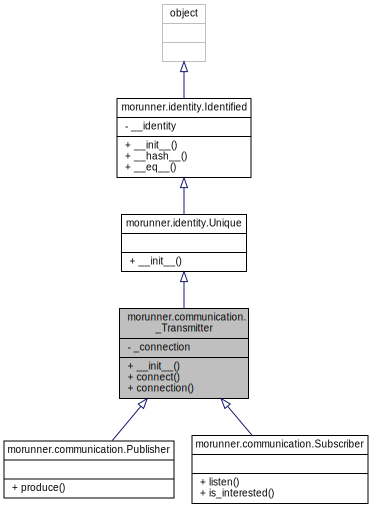
\includegraphics[width=350pt]{classmorunner_1_1communication_1_1__Transmitter__inherit__graph}
\end{center}
\end{figure}


Collaboration diagram for morunner.\+communication.\+\_\+\+Transmitter\+:
\nopagebreak
\begin{figure}[H]
\begin{center}
\leavevmode
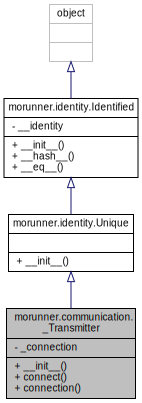
\includegraphics[width=214pt]{classmorunner_1_1communication_1_1__Transmitter__coll__graph}
\end{center}
\end{figure}
\subsection*{Public Member Functions}
\begin{DoxyCompactItemize}
\item 
def \hyperlink{classmorunner_1_1communication_1_1__Transmitter_ada6f89d3536ac6aeb6fe09fb3f5ac46e}{\+\_\+\+\_\+init\+\_\+\+\_\+} (self)
\item 
def \hyperlink{classmorunner_1_1communication_1_1__Transmitter_ad4e197abeee1bb81d41f57282ffb29c0}{connect}
\item 
def \hyperlink{classmorunner_1_1communication_1_1__Transmitter_a054317d3dbeecd42d6bbb81612d67ea5}{connection} (self)
\end{DoxyCompactItemize}
\subsection*{Private Attributes}
\begin{DoxyCompactItemize}
\item 
\hyperlink{classmorunner_1_1communication_1_1__Transmitter_a759fb3f16daa3686e84a775f6cb8e60d}{\+\_\+connection}
\end{DoxyCompactItemize}


\subsection{Detailed Description}


Definition at line 127 of file communication.\+py.



\subsection{Constructor \& Destructor Documentation}
\hypertarget{classmorunner_1_1communication_1_1__Transmitter_ada6f89d3536ac6aeb6fe09fb3f5ac46e}{}\index{morunner\+::communication\+::\+\_\+\+Transmitter@{morunner\+::communication\+::\+\_\+\+Transmitter}!\+\_\+\+\_\+init\+\_\+\+\_\+@{\+\_\+\+\_\+init\+\_\+\+\_\+}}
\index{\+\_\+\+\_\+init\+\_\+\+\_\+@{\+\_\+\+\_\+init\+\_\+\+\_\+}!morunner\+::communication\+::\+\_\+\+Transmitter@{morunner\+::communication\+::\+\_\+\+Transmitter}}
\subsubsection[{\+\_\+\+\_\+init\+\_\+\+\_\+(self)}]{\setlength{\rightskip}{0pt plus 5cm}def morunner.\+communication.\+\_\+\+Transmitter.\+\_\+\+\_\+init\+\_\+\+\_\+ (
\begin{DoxyParamCaption}
\item[{}]{self, }
\item[{}]{None}
\end{DoxyParamCaption}
)}\label{classmorunner_1_1communication_1_1__Transmitter_ada6f89d3536ac6aeb6fe09fb3f5ac46e}


Definition at line 129 of file communication.\+py.


\begin{DoxyCode}
129     \textcolor{keyword}{def }\hyperlink{classmorunner_1_1communication_1_1__Transmitter_ada6f89d3536ac6aeb6fe09fb3f5ac46e}{\_\_init\_\_}(self) -> None:
130         super().\hyperlink{classmorunner_1_1communication_1_1__Transmitter_ada6f89d3536ac6aeb6fe09fb3f5ac46e}{\_\_init\_\_}()
131         self.\hyperlink{classmorunner_1_1communication_1_1__Transmitter_a759fb3f16daa3686e84a775f6cb8e60d}{\_connection} = \textcolor{keywordtype}{None}
132 
\end{DoxyCode}


\subsection{Member Function Documentation}
\hypertarget{classmorunner_1_1communication_1_1__Transmitter_ad4e197abeee1bb81d41f57282ffb29c0}{}\index{morunner\+::communication\+::\+\_\+\+Transmitter@{morunner\+::communication\+::\+\_\+\+Transmitter}!connect@{connect}}
\index{connect@{connect}!morunner\+::communication\+::\+\_\+\+Transmitter@{morunner\+::communication\+::\+\_\+\+Transmitter}}
\subsubsection[{connect}]{\setlength{\rightskip}{0pt plus 5cm}def morunner.\+communication.\+\_\+\+Transmitter.\+connect (
\begin{DoxyParamCaption}
\item[{}]{self, }
\item[{}]{connection}
\end{DoxyParamCaption}
)}\label{classmorunner_1_1communication_1_1__Transmitter_ad4e197abeee1bb81d41f57282ffb29c0}


Definition at line 134 of file communication.\+py.



References morunner.\+communication.\+\_\+\+Transmitter.\+\_\+connection.


\begin{DoxyCode}
134                 connection: multiprocessing.connection.Connection
135                ) -> \textcolor{keywordtype}{None}:
136         self.\hyperlink{classmorunner_1_1communication_1_1__Transmitter_a759fb3f16daa3686e84a775f6cb8e60d}{\_connection} = connection
137 
\end{DoxyCode}
\hypertarget{classmorunner_1_1communication_1_1__Transmitter_a054317d3dbeecd42d6bbb81612d67ea5}{}\index{morunner\+::communication\+::\+\_\+\+Transmitter@{morunner\+::communication\+::\+\_\+\+Transmitter}!connection@{connection}}
\index{connection@{connection}!morunner\+::communication\+::\+\_\+\+Transmitter@{morunner\+::communication\+::\+\_\+\+Transmitter}}
\subsubsection[{connection(self)}]{\setlength{\rightskip}{0pt plus 5cm}def morunner.\+communication.\+\_\+\+Transmitter.\+connection (
\begin{DoxyParamCaption}
\item[{}]{self}
\end{DoxyParamCaption}
)}\label{classmorunner_1_1communication_1_1__Transmitter_a054317d3dbeecd42d6bbb81612d67ea5}


Definition at line 139 of file communication.\+py.



References morunner.\+communication.\+\_\+\+Transmitter.\+\_\+connection.



Referenced by morunner.\+communication.\+Subscriber.\+listen(), and morunner.\+communication.\+Publisher.\+produce().


\begin{DoxyCode}
139     \textcolor{keyword}{def }\hyperlink{classmorunner_1_1communication_1_1__Transmitter_a054317d3dbeecd42d6bbb81612d67ea5}{connection}(self):
140         \textcolor{keywordflow}{return} self.\hyperlink{classmorunner_1_1communication_1_1__Transmitter_a759fb3f16daa3686e84a775f6cb8e60d}{\_connection}
141 
142 
\end{DoxyCode}


Here is the caller graph for this function\+:
\nopagebreak
\begin{figure}[H]
\begin{center}
\leavevmode
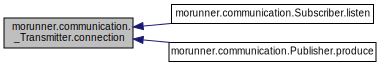
\includegraphics[width=350pt]{classmorunner_1_1communication_1_1__Transmitter_a054317d3dbeecd42d6bbb81612d67ea5_icgraph}
\end{center}
\end{figure}




\subsection{Member Data Documentation}
\hypertarget{classmorunner_1_1communication_1_1__Transmitter_a759fb3f16daa3686e84a775f6cb8e60d}{}\index{morunner\+::communication\+::\+\_\+\+Transmitter@{morunner\+::communication\+::\+\_\+\+Transmitter}!\+\_\+connection@{\+\_\+connection}}
\index{\+\_\+connection@{\+\_\+connection}!morunner\+::communication\+::\+\_\+\+Transmitter@{morunner\+::communication\+::\+\_\+\+Transmitter}}
\subsubsection[{\+\_\+connection}]{\setlength{\rightskip}{0pt plus 5cm}morunner.\+communication.\+\_\+\+Transmitter.\+\_\+connection\hspace{0.3cm}{\ttfamily [private]}}\label{classmorunner_1_1communication_1_1__Transmitter_a759fb3f16daa3686e84a775f6cb8e60d}


Definition at line 131 of file communication.\+py.



Referenced by morunner.\+communication.\+\_\+\+Transmitter.\+connect(), and morunner.\+communication.\+\_\+\+Transmitter.\+connection().



The documentation for this class was generated from the following file\+:\begin{DoxyCompactItemize}
\item 
src/morunner/\hyperlink{communication_8py}{communication.\+py}\end{DoxyCompactItemize}

\hypertarget{classmorunner_1_1communication_1_1Action}{}\section{morunner.\+communication.\+Action Class Reference}
\label{classmorunner_1_1communication_1_1Action}\index{morunner.\+communication.\+Action@{morunner.\+communication.\+Action}}


Inheritance diagram for morunner.\+communication.\+Action\+:
\nopagebreak
\begin{figure}[H]
\begin{center}
\leavevmode
\includegraphics[width=237pt]{classmorunner_1_1communication_1_1Action__inherit__graph}
\end{center}
\end{figure}


Collaboration diagram for morunner.\+communication.\+Action\+:
\nopagebreak
\begin{figure}[H]
\begin{center}
\leavevmode
\includegraphics[width=237pt]{classmorunner_1_1communication_1_1Action__coll__graph}
\end{center}
\end{figure}
\subsection*{Static Public Attributes}
\begin{DoxyCompactItemize}
\item 
int \hyperlink{classmorunner_1_1communication_1_1Action_a367a02befe76df874fe36b7342873f88}{discovery} = 1
\item 
int \hyperlink{classmorunner_1_1communication_1_1Action_a9e067338328ab2a5f6084c24b6091e0c}{read} = 2
\item 
int \hyperlink{classmorunner_1_1communication_1_1Action_aed47c16770d1f072b7a7d5bb6bfc0e13}{write} = 3
\item 
int \hyperlink{classmorunner_1_1communication_1_1Action_a4ecc5485449669bbd974615fe783577d}{initialize} = 4
\item 
int \hyperlink{classmorunner_1_1communication_1_1Action_aa749211a8116f9320662c45442f2b09f}{destroy} = 5
\item 
int \hyperlink{classmorunner_1_1communication_1_1Action_a0eac527678033a524b4077972d1450b4}{allocation} = 6
\item 
int \hyperlink{classmorunner_1_1communication_1_1Action_ad318c65952cf6ea310ffe8a755ae822c}{deallocation} = 7
\end{DoxyCompactItemize}


\subsection{Detailed Description}
\begin{DoxyVerb}The list of valid action codes for messages.
\end{DoxyVerb}
 

Definition at line 54 of file communication.\+py.



\subsection{Member Data Documentation}
\hypertarget{classmorunner_1_1communication_1_1Action_a0eac527678033a524b4077972d1450b4}{}\index{morunner\+::communication\+::\+Action@{morunner\+::communication\+::\+Action}!allocation@{allocation}}
\index{allocation@{allocation}!morunner\+::communication\+::\+Action@{morunner\+::communication\+::\+Action}}
\subsubsection[{allocation}]{\setlength{\rightskip}{0pt plus 5cm}int morunner.\+communication.\+Action.\+allocation = 6\hspace{0.3cm}{\ttfamily [static]}}\label{classmorunner_1_1communication_1_1Action_a0eac527678033a524b4077972d1450b4}


Definition at line 64 of file communication.\+py.

\hypertarget{classmorunner_1_1communication_1_1Action_ad318c65952cf6ea310ffe8a755ae822c}{}\index{morunner\+::communication\+::\+Action@{morunner\+::communication\+::\+Action}!deallocation@{deallocation}}
\index{deallocation@{deallocation}!morunner\+::communication\+::\+Action@{morunner\+::communication\+::\+Action}}
\subsubsection[{deallocation}]{\setlength{\rightskip}{0pt plus 5cm}int morunner.\+communication.\+Action.\+deallocation = 7\hspace{0.3cm}{\ttfamily [static]}}\label{classmorunner_1_1communication_1_1Action_ad318c65952cf6ea310ffe8a755ae822c}


Definition at line 65 of file communication.\+py.

\hypertarget{classmorunner_1_1communication_1_1Action_aa749211a8116f9320662c45442f2b09f}{}\index{morunner\+::communication\+::\+Action@{morunner\+::communication\+::\+Action}!destroy@{destroy}}
\index{destroy@{destroy}!morunner\+::communication\+::\+Action@{morunner\+::communication\+::\+Action}}
\subsubsection[{destroy}]{\setlength{\rightskip}{0pt plus 5cm}int morunner.\+communication.\+Action.\+destroy = 5\hspace{0.3cm}{\ttfamily [static]}}\label{classmorunner_1_1communication_1_1Action_aa749211a8116f9320662c45442f2b09f}


Definition at line 63 of file communication.\+py.

\hypertarget{classmorunner_1_1communication_1_1Action_a367a02befe76df874fe36b7342873f88}{}\index{morunner\+::communication\+::\+Action@{morunner\+::communication\+::\+Action}!discovery@{discovery}}
\index{discovery@{discovery}!morunner\+::communication\+::\+Action@{morunner\+::communication\+::\+Action}}
\subsubsection[{discovery}]{\setlength{\rightskip}{0pt plus 5cm}int morunner.\+communication.\+Action.\+discovery = 1\hspace{0.3cm}{\ttfamily [static]}}\label{classmorunner_1_1communication_1_1Action_a367a02befe76df874fe36b7342873f88}


Definition at line 59 of file communication.\+py.

\hypertarget{classmorunner_1_1communication_1_1Action_a4ecc5485449669bbd974615fe783577d}{}\index{morunner\+::communication\+::\+Action@{morunner\+::communication\+::\+Action}!initialize@{initialize}}
\index{initialize@{initialize}!morunner\+::communication\+::\+Action@{morunner\+::communication\+::\+Action}}
\subsubsection[{initialize}]{\setlength{\rightskip}{0pt plus 5cm}int morunner.\+communication.\+Action.\+initialize = 4\hspace{0.3cm}{\ttfamily [static]}}\label{classmorunner_1_1communication_1_1Action_a4ecc5485449669bbd974615fe783577d}


Definition at line 62 of file communication.\+py.

\hypertarget{classmorunner_1_1communication_1_1Action_a9e067338328ab2a5f6084c24b6091e0c}{}\index{morunner\+::communication\+::\+Action@{morunner\+::communication\+::\+Action}!read@{read}}
\index{read@{read}!morunner\+::communication\+::\+Action@{morunner\+::communication\+::\+Action}}
\subsubsection[{read}]{\setlength{\rightskip}{0pt plus 5cm}int morunner.\+communication.\+Action.\+read = 2\hspace{0.3cm}{\ttfamily [static]}}\label{classmorunner_1_1communication_1_1Action_a9e067338328ab2a5f6084c24b6091e0c}


Definition at line 60 of file communication.\+py.

\hypertarget{classmorunner_1_1communication_1_1Action_aed47c16770d1f072b7a7d5bb6bfc0e13}{}\index{morunner\+::communication\+::\+Action@{morunner\+::communication\+::\+Action}!write@{write}}
\index{write@{write}!morunner\+::communication\+::\+Action@{morunner\+::communication\+::\+Action}}
\subsubsection[{write}]{\setlength{\rightskip}{0pt plus 5cm}int morunner.\+communication.\+Action.\+write = 3\hspace{0.3cm}{\ttfamily [static]}}\label{classmorunner_1_1communication_1_1Action_aed47c16770d1f072b7a7d5bb6bfc0e13}


Definition at line 61 of file communication.\+py.



The documentation for this class was generated from the following file\+:\begin{DoxyCompactItemize}
\item 
src/morunner/\hyperlink{communication_8py}{communication.\+py}\end{DoxyCompactItemize}

\hypertarget{classmorunner_1_1break_1_1Break}{}\section{morunner.\+break.\+Break Class Reference}
\label{classmorunner_1_1break_1_1Break}\index{morunner.\+break.\+Break@{morunner.\+break.\+Break}}


Inheritance diagram for morunner.\+break.\+Break\+:
\nopagebreak
\begin{figure}[H]
\begin{center}
\leavevmode
\includegraphics[width=193pt]{classmorunner_1_1break_1_1Break__inherit__graph}
\end{center}
\end{figure}


Collaboration diagram for morunner.\+break.\+Break\+:
\nopagebreak
\begin{figure}[H]
\begin{center}
\leavevmode
\includegraphics[width=193pt]{classmorunner_1_1break_1_1Break__coll__graph}
\end{center}
\end{figure}
\subsection*{Public Member Functions}
\begin{DoxyCompactItemize}
\item 
def \hyperlink{classmorunner_1_1break_1_1Break_ad40ba1a8f3e8eb89cf2b49272637af15}{\+\_\+\+\_\+init\+\_\+\+\_\+}
\item 
def \hyperlink{classmorunner_1_1break_1_1Break_aa753a1991e864f09e5c88fa091045a54}{add\+\_\+task} (self, task)
\item 
def \hyperlink{classmorunner_1_1break_1_1Break_a751c8b40ea48a5119871d370e8ed3105}{add\+\_\+tasks} (self, \hyperlink{classmorunner_1_1break_1_1Break_a7d62d6a7a0f7f526ca0a15363eda01d6}{tasks})
\item 
def \hyperlink{classmorunner_1_1break_1_1Break_ae53ddba489aac5ad45172f9c4ad6f634}{stop} (self)
\end{DoxyCompactItemize}
\subsection*{Public Attributes}
\begin{DoxyCompactItemize}
\item 
\hyperlink{classmorunner_1_1break_1_1Break_a4f411d3199721dd388f4511d4075a0cc}{silent}
\item 
\hyperlink{classmorunner_1_1break_1_1Break_a0ca27884fb0c27084b04fb7ab17a7476}{enabled}
\item 
\hyperlink{classmorunner_1_1break_1_1Break_a7d62d6a7a0f7f526ca0a15363eda01d6}{tasks}
\end{DoxyCompactItemize}


\subsection{Detailed Description}


Definition at line 31 of file break.\+py.



\subsection{Constructor \& Destructor Documentation}
\hypertarget{classmorunner_1_1break_1_1Break_ad40ba1a8f3e8eb89cf2b49272637af15}{}\index{morunner\+::break\+::\+Break@{morunner\+::break\+::\+Break}!\+\_\+\+\_\+init\+\_\+\+\_\+@{\+\_\+\+\_\+init\+\_\+\+\_\+}}
\index{\+\_\+\+\_\+init\+\_\+\+\_\+@{\+\_\+\+\_\+init\+\_\+\+\_\+}!morunner\+::break\+::\+Break@{morunner\+::break\+::\+Break}}
\subsubsection[{\+\_\+\+\_\+init\+\_\+\+\_\+}]{\setlength{\rightskip}{0pt plus 5cm}def morunner.\+break.\+Break.\+\_\+\+\_\+init\+\_\+\+\_\+ (
\begin{DoxyParamCaption}
\item[{}]{self, }
\item[{}]{condition}
\end{DoxyParamCaption}
)}\label{classmorunner_1_1break_1_1Break_ad40ba1a8f3e8eb89cf2b49272637af15}


Definition at line 33 of file break.\+py.


\begin{DoxyCode}
33     \textcolor{keyword}{def }\hyperlink{classmorunner_1_1break_1_1Break_ad40ba1a8f3e8eb89cf2b49272637af15}{\_\_init\_\_}(self, condition: BreakCondition) -> \textcolor{keywordtype}{None}:
34         super(Break, self).\hyperlink{classmorunner_1_1break_1_1Break_ad40ba1a8f3e8eb89cf2b49272637af15}{\_\_init\_\_}(*condition)
35         self.\hyperlink{classmorunner_1_1break_1_1Break_a4f411d3199721dd388f4511d4075a0cc}{silent} = \textcolor{keyword}{True}
36         self.\hyperlink{classmorunner_1_1break_1_1Break_a0ca27884fb0c27084b04fb7ab17a7476}{enabled} = \textcolor{keyword}{True}
37         self.\hyperlink{classmorunner_1_1break_1_1Break_a7d62d6a7a0f7f526ca0a15363eda01d6}{tasks} = set()
38 
\end{DoxyCode}


\subsection{Member Function Documentation}
\hypertarget{classmorunner_1_1break_1_1Break_aa753a1991e864f09e5c88fa091045a54}{}\index{morunner\+::break\+::\+Break@{morunner\+::break\+::\+Break}!add\+\_\+task@{add\+\_\+task}}
\index{add\+\_\+task@{add\+\_\+task}!morunner\+::break\+::\+Break@{morunner\+::break\+::\+Break}}
\subsubsection[{add\+\_\+task(self, task)}]{\setlength{\rightskip}{0pt plus 5cm}def morunner.\+break.\+Break.\+add\+\_\+task (
\begin{DoxyParamCaption}
\item[{}]{self, }
\item[{}]{task, }
\item[{}]{None}
\end{DoxyParamCaption}
)}\label{classmorunner_1_1break_1_1Break_aa753a1991e864f09e5c88fa091045a54}


Definition at line 39 of file break.\+py.


\begin{DoxyCode}
39     \textcolor{keyword}{def }\hyperlink{classmorunner_1_1break_1_1Break_aa753a1991e864f09e5c88fa091045a54}{add\_task}(self, task) -> None:
40         self.tasks.add(task)
41 
\end{DoxyCode}
\hypertarget{classmorunner_1_1break_1_1Break_a751c8b40ea48a5119871d370e8ed3105}{}\index{morunner\+::break\+::\+Break@{morunner\+::break\+::\+Break}!add\+\_\+tasks@{add\+\_\+tasks}}
\index{add\+\_\+tasks@{add\+\_\+tasks}!morunner\+::break\+::\+Break@{morunner\+::break\+::\+Break}}
\subsubsection[{add\+\_\+tasks(self, tasks)}]{\setlength{\rightskip}{0pt plus 5cm}def morunner.\+break.\+Break.\+add\+\_\+tasks (
\begin{DoxyParamCaption}
\item[{}]{self, }
\item[{}]{tasks}
\end{DoxyParamCaption}
)}\label{classmorunner_1_1break_1_1Break_a751c8b40ea48a5119871d370e8ed3105}


Definition at line 42 of file break.\+py.


\begin{DoxyCode}
42     \textcolor{keyword}{def }\hyperlink{classmorunner_1_1break_1_1Break_a751c8b40ea48a5119871d370e8ed3105}{add\_tasks}(self, tasks):
43         self.tasks.update(tasks)
44 
\end{DoxyCode}
\hypertarget{classmorunner_1_1break_1_1Break_ae53ddba489aac5ad45172f9c4ad6f634}{}\index{morunner\+::break\+::\+Break@{morunner\+::break\+::\+Break}!stop@{stop}}
\index{stop@{stop}!morunner\+::break\+::\+Break@{morunner\+::break\+::\+Break}}
\subsubsection[{stop(self)}]{\setlength{\rightskip}{0pt plus 5cm}def morunner.\+break.\+Break.\+stop (
\begin{DoxyParamCaption}
\item[{}]{self}
\end{DoxyParamCaption}
)}\label{classmorunner_1_1break_1_1Break_ae53ddba489aac5ad45172f9c4ad6f634}


Definition at line 45 of file break.\+py.



References morunner.\+break.\+Break.\+tasks.


\begin{DoxyCode}
45     \textcolor{keyword}{def }\hyperlink{classmorunner_1_1break_1_1Break_ae53ddba489aac5ad45172f9c4ad6f634}{stop}(self):
46         frame = gdb.newest\_frame()
47         \textcolor{keywordflow}{for} task \textcolor{keywordflow}{in} self.\hyperlink{classmorunner_1_1break_1_1Break_a7d62d6a7a0f7f526ca0a15363eda01d6}{tasks}:
48             task.run(frame)
49         \textcolor{keywordflow}{return} \textcolor{keyword}{False}
50 
51 \end{DoxyCode}


\subsection{Member Data Documentation}
\hypertarget{classmorunner_1_1break_1_1Break_a0ca27884fb0c27084b04fb7ab17a7476}{}\index{morunner\+::break\+::\+Break@{morunner\+::break\+::\+Break}!enabled@{enabled}}
\index{enabled@{enabled}!morunner\+::break\+::\+Break@{morunner\+::break\+::\+Break}}
\subsubsection[{enabled}]{\setlength{\rightskip}{0pt plus 5cm}morunner.\+break.\+Break.\+enabled}\label{classmorunner_1_1break_1_1Break_a0ca27884fb0c27084b04fb7ab17a7476}


Definition at line 36 of file break.\+py.

\hypertarget{classmorunner_1_1break_1_1Break_a4f411d3199721dd388f4511d4075a0cc}{}\index{morunner\+::break\+::\+Break@{morunner\+::break\+::\+Break}!silent@{silent}}
\index{silent@{silent}!morunner\+::break\+::\+Break@{morunner\+::break\+::\+Break}}
\subsubsection[{silent}]{\setlength{\rightskip}{0pt plus 5cm}morunner.\+break.\+Break.\+silent}\label{classmorunner_1_1break_1_1Break_a4f411d3199721dd388f4511d4075a0cc}


Definition at line 35 of file break.\+py.

\hypertarget{classmorunner_1_1break_1_1Break_a7d62d6a7a0f7f526ca0a15363eda01d6}{}\index{morunner\+::break\+::\+Break@{morunner\+::break\+::\+Break}!tasks@{tasks}}
\index{tasks@{tasks}!morunner\+::break\+::\+Break@{morunner\+::break\+::\+Break}}
\subsubsection[{tasks}]{\setlength{\rightskip}{0pt plus 5cm}morunner.\+break.\+Break.\+tasks}\label{classmorunner_1_1break_1_1Break_a7d62d6a7a0f7f526ca0a15363eda01d6}


Definition at line 37 of file break.\+py.



Referenced by morunner.\+break.\+Break.\+stop().



The documentation for this class was generated from the following file\+:\begin{DoxyCompactItemize}
\item 
src/morunner/\hyperlink{break_8py}{break.\+py}\end{DoxyCompactItemize}

\input{classmorunner_1_1communication_1_1Broadcaster}
\hypertarget{classmorunner_1_1identity_1_1Identified}{}\section{morunner.\+identity.\+Identified Class Reference}
\label{classmorunner_1_1identity_1_1Identified}\index{morunner.\+identity.\+Identified@{morunner.\+identity.\+Identified}}


Inheritance diagram for morunner.\+identity.\+Identified\+:
\nopagebreak
\begin{figure}[H]
\begin{center}
\leavevmode
\includegraphics[width=350pt]{classmorunner_1_1identity_1_1Identified__inherit__graph}
\end{center}
\end{figure}


Collaboration diagram for morunner.\+identity.\+Identified\+:
\nopagebreak
\begin{figure}[H]
\begin{center}
\leavevmode
\includegraphics[width=214pt]{classmorunner_1_1identity_1_1Identified__coll__graph}
\end{center}
\end{figure}
\subsection*{Public Member Functions}
\begin{DoxyCompactItemize}
\item 
def \hyperlink{classmorunner_1_1identity_1_1Identified_a80d2a5b6cbcd0a973dc4739b82dde0e4}{\+\_\+\+\_\+init\+\_\+\+\_\+}
\item 
def \hyperlink{classmorunner_1_1identity_1_1Identified_a8dc07b6cab1347c13604ec590fde6be7}{\+\_\+\+\_\+hash\+\_\+\+\_\+} (self)
\item 
def \hyperlink{classmorunner_1_1identity_1_1Identified_ace36100c76bb00edaa564fb8548cf5aa}{\+\_\+\+\_\+eq\+\_\+\+\_\+}
\end{DoxyCompactItemize}
\subsection*{Private Attributes}
\begin{DoxyCompactItemize}
\item 
\hyperlink{classmorunner_1_1identity_1_1Identified_ac77d666680df7ce36c8839b6bb61a4d6}{\+\_\+\+\_\+identity}
\end{DoxyCompactItemize}


\subsection{Detailed Description}
\begin{DoxyVerb}Identified is a base class for other identity classes in this module.  You
can directly use it to define other identity classes if you like, but try
not to rely on its internal mechanics, as these are far from final.

The goal of this  is to prevent the user from even needing to consider
the means by which the identity is assigned, the member variable to which
it is assigned, or anything about it.  Please do not attempt to even access
the identity value.  Just use the hash function if you truly need a unique
id number for your object, as the identity implementation could (in theory)
change in incompatible ways.
\end{DoxyVerb}
 

Definition at line 14 of file identity.\+py.



\subsection{Constructor \& Destructor Documentation}
\hypertarget{classmorunner_1_1identity_1_1Identified_a80d2a5b6cbcd0a973dc4739b82dde0e4}{}\index{morunner\+::identity\+::\+Identified@{morunner\+::identity\+::\+Identified}!\+\_\+\+\_\+init\+\_\+\+\_\+@{\+\_\+\+\_\+init\+\_\+\+\_\+}}
\index{\+\_\+\+\_\+init\+\_\+\+\_\+@{\+\_\+\+\_\+init\+\_\+\+\_\+}!morunner\+::identity\+::\+Identified@{morunner\+::identity\+::\+Identified}}
\subsubsection[{\+\_\+\+\_\+init\+\_\+\+\_\+}]{\setlength{\rightskip}{0pt plus 5cm}def morunner.\+identity.\+Identified.\+\_\+\+\_\+init\+\_\+\+\_\+ (
\begin{DoxyParamCaption}
\item[{}]{self, }
\item[{}]{identity\+\_\+function}
\end{DoxyParamCaption}
)}\label{classmorunner_1_1identity_1_1Identified_a80d2a5b6cbcd0a973dc4739b82dde0e4}


Definition at line 29 of file identity.\+py.


\begin{DoxyCode}
29                  identity\_function: typing.Callable[[], typing.Hashable[object]]
30                 ) -> \textcolor{keywordtype}{None}:
31         \textcolor{stringliteral}{"""}
32 \textcolor{stringliteral}{        Invoke identity\_function to construct the identity of this instance.}
33 \textcolor{stringliteral}{}
34 \textcolor{stringliteral}{        @param identity\_function a nullary function used to assign an identity}
35 \textcolor{stringliteral}{        to this instance.}
36 \textcolor{stringliteral}{        """}
37         self.\hyperlink{classmorunner_1_1identity_1_1Identified_ac77d666680df7ce36c8839b6bb61a4d6}{\_\_identity} = hash(identity\_function())
38 
\end{DoxyCode}


\subsection{Member Function Documentation}
\hypertarget{classmorunner_1_1identity_1_1Identified_ace36100c76bb00edaa564fb8548cf5aa}{}\index{morunner\+::identity\+::\+Identified@{morunner\+::identity\+::\+Identified}!\+\_\+\+\_\+eq\+\_\+\+\_\+@{\+\_\+\+\_\+eq\+\_\+\+\_\+}}
\index{\+\_\+\+\_\+eq\+\_\+\+\_\+@{\+\_\+\+\_\+eq\+\_\+\+\_\+}!morunner\+::identity\+::\+Identified@{morunner\+::identity\+::\+Identified}}
\subsubsection[{\+\_\+\+\_\+eq\+\_\+\+\_\+}]{\setlength{\rightskip}{0pt plus 5cm}def morunner.\+identity.\+Identified.\+\_\+\+\_\+eq\+\_\+\+\_\+ (
\begin{DoxyParamCaption}
\item[{}]{self, }
\item[{}]{rhs}
\end{DoxyParamCaption}
)}\label{classmorunner_1_1identity_1_1Identified_ace36100c76bb00edaa564fb8548cf5aa}


Definition at line 48 of file identity.\+py.


\begin{DoxyCode}
48     \textcolor{keyword}{def }\hyperlink{classmorunner_1_1identity_1_1Identified_ace36100c76bb00edaa564fb8548cf5aa}{\_\_eq\_\_}(self, rhs: \textcolor{stringliteral}{'Identified'}) -> bool:
49         \textcolor{stringliteral}{"""}
50 \textcolor{stringliteral}{        Equivalence check between two Identified objects.}
51 \textcolor{stringliteral}{}
52 \textcolor{stringliteral}{        @return <bool> The equivalence of self and rhs.}
53 \textcolor{stringliteral}{        """}
54         \textcolor{keywordflow}{return} isinstance(rhs, Identified) \textcolor{keywordflow}{and} (hash(self) == hash(rhs))
55 
56 
57 
\end{DoxyCode}
\hypertarget{classmorunner_1_1identity_1_1Identified_a8dc07b6cab1347c13604ec590fde6be7}{}\index{morunner\+::identity\+::\+Identified@{morunner\+::identity\+::\+Identified}!\+\_\+\+\_\+hash\+\_\+\+\_\+@{\+\_\+\+\_\+hash\+\_\+\+\_\+}}
\index{\+\_\+\+\_\+hash\+\_\+\+\_\+@{\+\_\+\+\_\+hash\+\_\+\+\_\+}!morunner\+::identity\+::\+Identified@{morunner\+::identity\+::\+Identified}}
\subsubsection[{\+\_\+\+\_\+hash\+\_\+\+\_\+(self)}]{\setlength{\rightskip}{0pt plus 5cm}def morunner.\+identity.\+Identified.\+\_\+\+\_\+hash\+\_\+\+\_\+ (
\begin{DoxyParamCaption}
\item[{}]{self, }
\item[{}]{int}
\end{DoxyParamCaption}
)}\label{classmorunner_1_1identity_1_1Identified_a8dc07b6cab1347c13604ec590fde6be7}
\begin{DoxyVerb}Return a hash which is *only* a function of the identity assigned at
__init__.

@return <int> The hash of the value returned by identity_function() at init.
\end{DoxyVerb}
 

Definition at line 39 of file identity.\+py.



References morunner.\+identity.\+Identified.\+\_\+\+\_\+identity.


\begin{DoxyCode}
39     \textcolor{keyword}{def }\hyperlink{classmorunner_1_1identity_1_1Identified_a8dc07b6cab1347c13604ec590fde6be7}{\_\_hash\_\_}(self) -> int:
40         \textcolor{stringliteral}{"""}
41 \textcolor{stringliteral}{        Return a hash which is *only* a function of the identity assigned at}
42 \textcolor{stringliteral}{        \_\_init\_\_.}
43 \textcolor{stringliteral}{}
44 \textcolor{stringliteral}{        @return <int> The hash of the value returned by identity\_function() at init.}
45 \textcolor{stringliteral}{        """}
46         \textcolor{keywordflow}{return} self.\hyperlink{classmorunner_1_1identity_1_1Identified_ac77d666680df7ce36c8839b6bb61a4d6}{\_\_identity}
47 
\end{DoxyCode}


\subsection{Member Data Documentation}
\hypertarget{classmorunner_1_1identity_1_1Identified_ac77d666680df7ce36c8839b6bb61a4d6}{}\index{morunner\+::identity\+::\+Identified@{morunner\+::identity\+::\+Identified}!\+\_\+\+\_\+identity@{\+\_\+\+\_\+identity}}
\index{\+\_\+\+\_\+identity@{\+\_\+\+\_\+identity}!morunner\+::identity\+::\+Identified@{morunner\+::identity\+::\+Identified}}
\subsubsection[{\+\_\+\+\_\+identity}]{\setlength{\rightskip}{0pt plus 5cm}morunner.\+identity.\+Identified.\+\_\+\+\_\+identity\hspace{0.3cm}{\ttfamily [private]}}\label{classmorunner_1_1identity_1_1Identified_ac77d666680df7ce36c8839b6bb61a4d6}


Definition at line 37 of file identity.\+py.



Referenced by morunner.\+identity.\+Identified.\+\_\+\+\_\+hash\+\_\+\+\_\+().



The documentation for this class was generated from the following file\+:\begin{DoxyCompactItemize}
\item 
src/morunner/\hyperlink{identity_8py}{identity.\+py}\end{DoxyCompactItemize}

\hypertarget{classmorunner_1_1communication_1_1Message}{}\section{morunner.\+communication.\+Message Class Reference}
\label{classmorunner_1_1communication_1_1Message}\index{morunner.\+communication.\+Message@{morunner.\+communication.\+Message}}


Inheritance diagram for morunner.\+communication.\+Message\+:
\nopagebreak
\begin{figure}[H]
\begin{center}
\leavevmode
\includegraphics[width=249pt]{classmorunner_1_1communication_1_1Message__inherit__graph}
\end{center}
\end{figure}


Collaboration diagram for morunner.\+communication.\+Message\+:
\nopagebreak
\begin{figure}[H]
\begin{center}
\leavevmode
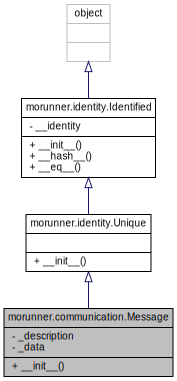
\includegraphics[width=249pt]{classmorunner_1_1communication_1_1Message__coll__graph}
\end{center}
\end{figure}
\subsection*{Public Member Functions}
\begin{DoxyCompactItemize}
\item 
def \hyperlink{classmorunner_1_1communication_1_1Message_a4f10c83eae9c4899e31ddae252687899}{\+\_\+\+\_\+init\+\_\+\+\_\+}
\end{DoxyCompactItemize}
\subsection*{Private Attributes}
\begin{DoxyCompactItemize}
\item 
\hyperlink{classmorunner_1_1communication_1_1Message_a7645e37f561610793530a6c329ab55fe}{\+\_\+description}
\item 
\hyperlink{classmorunner_1_1communication_1_1Message_a1735c0a988d7a81371b188d36913da1c}{\+\_\+data}
\end{DoxyCompactItemize}


\subsection{Detailed Description}
\begin{DoxyVerb}Message between components of the runner.
\end{DoxyVerb}
 

Definition at line 113 of file communication.\+py.



\subsection{Constructor \& Destructor Documentation}
\hypertarget{classmorunner_1_1communication_1_1Message_a4f10c83eae9c4899e31ddae252687899}{}\index{morunner\+::communication\+::\+Message@{morunner\+::communication\+::\+Message}!\+\_\+\+\_\+init\+\_\+\+\_\+@{\+\_\+\+\_\+init\+\_\+\+\_\+}}
\index{\+\_\+\+\_\+init\+\_\+\+\_\+@{\+\_\+\+\_\+init\+\_\+\+\_\+}!morunner\+::communication\+::\+Message@{morunner\+::communication\+::\+Message}}
\subsubsection[{\+\_\+\+\_\+init\+\_\+\+\_\+}]{\setlength{\rightskip}{0pt plus 5cm}def morunner.\+communication.\+Message.\+\_\+\+\_\+init\+\_\+\+\_\+ (
\begin{DoxyParamCaption}
\item[{}]{self, }
\item[{}]{description}
\end{DoxyParamCaption}
)}\label{classmorunner_1_1communication_1_1Message_a4f10c83eae9c4899e31ddae252687899}


Definition at line 119 of file communication.\+py.


\begin{DoxyCode}
119                  description: MessageDescription,
120                  data: object \textcolor{comment}{# NOTE: data must be pickleable!}
121                 ) -> \textcolor{keywordtype}{None}:
122         super().\hyperlink{classmorunner_1_1communication_1_1Message_a4f10c83eae9c4899e31ddae252687899}{\_\_init\_\_}()
123         self.\hyperlink{classmorunner_1_1communication_1_1Message_a7645e37f561610793530a6c329ab55fe}{\_description} = description
124         self.\hyperlink{classmorunner_1_1communication_1_1Message_a1735c0a988d7a81371b188d36913da1c}{\_data} = data
125 
126 
\end{DoxyCode}


\subsection{Member Data Documentation}
\hypertarget{classmorunner_1_1communication_1_1Message_a1735c0a988d7a81371b188d36913da1c}{}\index{morunner\+::communication\+::\+Message@{morunner\+::communication\+::\+Message}!\+\_\+data@{\+\_\+data}}
\index{\+\_\+data@{\+\_\+data}!morunner\+::communication\+::\+Message@{morunner\+::communication\+::\+Message}}
\subsubsection[{\+\_\+data}]{\setlength{\rightskip}{0pt plus 5cm}morunner.\+communication.\+Message.\+\_\+data\hspace{0.3cm}{\ttfamily [private]}}\label{classmorunner_1_1communication_1_1Message_a1735c0a988d7a81371b188d36913da1c}


Definition at line 124 of file communication.\+py.

\hypertarget{classmorunner_1_1communication_1_1Message_a7645e37f561610793530a6c329ab55fe}{}\index{morunner\+::communication\+::\+Message@{morunner\+::communication\+::\+Message}!\+\_\+description@{\+\_\+description}}
\index{\+\_\+description@{\+\_\+description}!morunner\+::communication\+::\+Message@{morunner\+::communication\+::\+Message}}
\subsubsection[{\+\_\+description}]{\setlength{\rightskip}{0pt plus 5cm}morunner.\+communication.\+Message.\+\_\+description\hspace{0.3cm}{\ttfamily [private]}}\label{classmorunner_1_1communication_1_1Message_a7645e37f561610793530a6c329ab55fe}


Definition at line 123 of file communication.\+py.



The documentation for this class was generated from the following file\+:\begin{DoxyCompactItemize}
\item 
src/morunner/\hyperlink{communication_8py}{communication.\+py}\end{DoxyCompactItemize}

\hypertarget{classmorunner_1_1communication_1_1MessageDescription}{}\section{morunner.\+communication.\+Message\+Description Class Reference}
\label{classmorunner_1_1communication_1_1MessageDescription}\index{morunner.\+communication.\+Message\+Description@{morunner.\+communication.\+Message\+Description}}


Inheritance diagram for morunner.\+communication.\+Message\+Description\+:
\nopagebreak
\begin{figure}[H]
\begin{center}
\leavevmode
\includegraphics[width=249pt]{classmorunner_1_1communication_1_1MessageDescription__inherit__graph}
\end{center}
\end{figure}


Collaboration diagram for morunner.\+communication.\+Message\+Description\+:
\nopagebreak
\begin{figure}[H]
\begin{center}
\leavevmode
\includegraphics[width=249pt]{classmorunner_1_1communication_1_1MessageDescription__coll__graph}
\end{center}
\end{figure}
\subsection*{Public Member Functions}
\begin{DoxyCompactItemize}
\item 
def \hyperlink{classmorunner_1_1communication_1_1MessageDescription_a98b5362654b69de4e75084a91fb75d76}{\+\_\+\+\_\+init\+\_\+\+\_\+}
\item 
def \hyperlink{classmorunner_1_1communication_1_1MessageDescription_ae8c519edd001e5382aaec99d953a8338}{action} (self)
\item 
def \hyperlink{classmorunner_1_1communication_1_1MessageDescription_ae52e8de1f7dd35cfb953deadbae19cc6}{subject} (self)
\end{DoxyCompactItemize}
\subsection*{Private Attributes}
\begin{DoxyCompactItemize}
\item 
\hyperlink{classmorunner_1_1communication_1_1MessageDescription_a812e6e0ac14765422a3b5c17443501d5}{\+\_\+action}
\item 
\hyperlink{classmorunner_1_1communication_1_1MessageDescription_abdd477c4b0afa84b46bd40b9f2f583c1}{\+\_\+subject}
\end{DoxyCompactItemize}


\subsection{Detailed Description}
\begin{DoxyVerb}Provides data about a message, which subscribers can use to decide if they
are "interested."
\end{DoxyVerb}
 

Definition at line 91 of file communication.\+py.



\subsection{Constructor \& Destructor Documentation}
\hypertarget{classmorunner_1_1communication_1_1MessageDescription_a98b5362654b69de4e75084a91fb75d76}{}\index{morunner\+::communication\+::\+Message\+Description@{morunner\+::communication\+::\+Message\+Description}!\+\_\+\+\_\+init\+\_\+\+\_\+@{\+\_\+\+\_\+init\+\_\+\+\_\+}}
\index{\+\_\+\+\_\+init\+\_\+\+\_\+@{\+\_\+\+\_\+init\+\_\+\+\_\+}!morunner\+::communication\+::\+Message\+Description@{morunner\+::communication\+::\+Message\+Description}}
\subsubsection[{\+\_\+\+\_\+init\+\_\+\+\_\+}]{\setlength{\rightskip}{0pt plus 5cm}def morunner.\+communication.\+Message\+Description.\+\_\+\+\_\+init\+\_\+\+\_\+ (
\begin{DoxyParamCaption}
\item[{}]{self, }
\item[{}]{action}
\end{DoxyParamCaption}
)}\label{classmorunner_1_1communication_1_1MessageDescription_a98b5362654b69de4e75084a91fb75d76}


Definition at line 98 of file communication.\+py.


\begin{DoxyCode}
98                  action: Action,
99                  subject: Subject
100                 ) -> \textcolor{keywordtype}{None}:
101         self.\hyperlink{classmorunner_1_1communication_1_1MessageDescription_a812e6e0ac14765422a3b5c17443501d5}{\_action} = action
102         self.\hyperlink{classmorunner_1_1communication_1_1MessageDescription_abdd477c4b0afa84b46bd40b9f2f583c1}{\_subject} = subject
103 
\end{DoxyCode}


\subsection{Member Function Documentation}
\hypertarget{classmorunner_1_1communication_1_1MessageDescription_ae8c519edd001e5382aaec99d953a8338}{}\index{morunner\+::communication\+::\+Message\+Description@{morunner\+::communication\+::\+Message\+Description}!action@{action}}
\index{action@{action}!morunner\+::communication\+::\+Message\+Description@{morunner\+::communication\+::\+Message\+Description}}
\subsubsection[{action(self)}]{\setlength{\rightskip}{0pt plus 5cm}def morunner.\+communication.\+Message\+Description.\+action (
\begin{DoxyParamCaption}
\item[{}]{self, }
\item[{}]{Action}
\end{DoxyParamCaption}
)}\label{classmorunner_1_1communication_1_1MessageDescription_ae8c519edd001e5382aaec99d953a8338}


Definition at line 105 of file communication.\+py.



References morunner.\+communication.\+Message\+Description.\+\_\+action.


\begin{DoxyCode}
105     \textcolor{keyword}{def }\hyperlink{classmorunner_1_1communication_1_1MessageDescription_ae8c519edd001e5382aaec99d953a8338}{action}(self) -> Action:
106         \textcolor{keywordflow}{return} self.\hyperlink{classmorunner_1_1communication_1_1MessageDescription_a812e6e0ac14765422a3b5c17443501d5}{\_action}
107 
\end{DoxyCode}
\hypertarget{classmorunner_1_1communication_1_1MessageDescription_ae52e8de1f7dd35cfb953deadbae19cc6}{}\index{morunner\+::communication\+::\+Message\+Description@{morunner\+::communication\+::\+Message\+Description}!subject@{subject}}
\index{subject@{subject}!morunner\+::communication\+::\+Message\+Description@{morunner\+::communication\+::\+Message\+Description}}
\subsubsection[{subject(self)}]{\setlength{\rightskip}{0pt plus 5cm}def morunner.\+communication.\+Message\+Description.\+subject (
\begin{DoxyParamCaption}
\item[{}]{self, }
\item[{}]{Subject}
\end{DoxyParamCaption}
)}\label{classmorunner_1_1communication_1_1MessageDescription_ae52e8de1f7dd35cfb953deadbae19cc6}


Definition at line 109 of file communication.\+py.



References morunner.\+communication.\+Message\+Description.\+\_\+subject.


\begin{DoxyCode}
109     \textcolor{keyword}{def }\hyperlink{classmorunner_1_1communication_1_1MessageDescription_ae52e8de1f7dd35cfb953deadbae19cc6}{subject}(self) -> Subject:
110         \textcolor{keywordflow}{return} self.\hyperlink{classmorunner_1_1communication_1_1MessageDescription_abdd477c4b0afa84b46bd40b9f2f583c1}{\_subject}
111 
112 
\end{DoxyCode}


\subsection{Member Data Documentation}
\hypertarget{classmorunner_1_1communication_1_1MessageDescription_a812e6e0ac14765422a3b5c17443501d5}{}\index{morunner\+::communication\+::\+Message\+Description@{morunner\+::communication\+::\+Message\+Description}!\+\_\+action@{\+\_\+action}}
\index{\+\_\+action@{\+\_\+action}!morunner\+::communication\+::\+Message\+Description@{morunner\+::communication\+::\+Message\+Description}}
\subsubsection[{\+\_\+action}]{\setlength{\rightskip}{0pt plus 5cm}morunner.\+communication.\+Message\+Description.\+\_\+action\hspace{0.3cm}{\ttfamily [private]}}\label{classmorunner_1_1communication_1_1MessageDescription_a812e6e0ac14765422a3b5c17443501d5}


Definition at line 101 of file communication.\+py.



Referenced by morunner.\+communication.\+Message\+Description.\+action().

\hypertarget{classmorunner_1_1communication_1_1MessageDescription_abdd477c4b0afa84b46bd40b9f2f583c1}{}\index{morunner\+::communication\+::\+Message\+Description@{morunner\+::communication\+::\+Message\+Description}!\+\_\+subject@{\+\_\+subject}}
\index{\+\_\+subject@{\+\_\+subject}!morunner\+::communication\+::\+Message\+Description@{morunner\+::communication\+::\+Message\+Description}}
\subsubsection[{\+\_\+subject}]{\setlength{\rightskip}{0pt plus 5cm}morunner.\+communication.\+Message\+Description.\+\_\+subject\hspace{0.3cm}{\ttfamily [private]}}\label{classmorunner_1_1communication_1_1MessageDescription_abdd477c4b0afa84b46bd40b9f2f583c1}


Definition at line 102 of file communication.\+py.



Referenced by morunner.\+communication.\+Message\+Description.\+subject().



The documentation for this class was generated from the following file\+:\begin{DoxyCompactItemize}
\item 
src/morunner/\hyperlink{communication_8py}{communication.\+py}\end{DoxyCompactItemize}

\hypertarget{classmorunner_1_1communication_1_1Publisher}{}\section{morunner.\+communication.\+Publisher Class Reference}
\label{classmorunner_1_1communication_1_1Publisher}\index{morunner.\+communication.\+Publisher@{morunner.\+communication.\+Publisher}}


Inheritance diagram for morunner.\+communication.\+Publisher\+:
\nopagebreak
\begin{figure}[H]
\begin{center}
\leavevmode
\includegraphics[height=550pt]{classmorunner_1_1communication_1_1Publisher__inherit__graph}
\end{center}
\end{figure}


Collaboration diagram for morunner.\+communication.\+Publisher\+:
\nopagebreak
\begin{figure}[H]
\begin{center}
\leavevmode
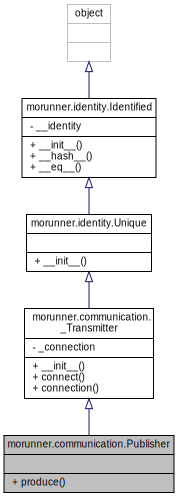
\includegraphics[height=550pt]{classmorunner_1_1communication_1_1Publisher__coll__graph}
\end{center}
\end{figure}
\subsection*{Public Member Functions}
\begin{DoxyCompactItemize}
\item 
def \hyperlink{classmorunner_1_1communication_1_1Publisher_a31e6bd7d0f60bfde37c026ddd55ff8b6}{produce}
\end{DoxyCompactItemize}


\subsection{Detailed Description}


Definition at line 143 of file communication.\+py.



\subsection{Member Function Documentation}
\hypertarget{classmorunner_1_1communication_1_1Publisher_a31e6bd7d0f60bfde37c026ddd55ff8b6}{}\index{morunner\+::communication\+::\+Publisher@{morunner\+::communication\+::\+Publisher}!produce@{produce}}
\index{produce@{produce}!morunner\+::communication\+::\+Publisher@{morunner\+::communication\+::\+Publisher}}
\subsubsection[{produce}]{\setlength{\rightskip}{0pt plus 5cm}def morunner.\+communication.\+Publisher.\+produce (
\begin{DoxyParamCaption}
\item[{}]{self, }
\item[{}]{message}
\end{DoxyParamCaption}
)}\label{classmorunner_1_1communication_1_1Publisher_a31e6bd7d0f60bfde37c026ddd55ff8b6}


Definition at line 145 of file communication.\+py.



References morunner.\+communication.\+\_\+\+Transmitter.\+connection().


\begin{DoxyCode}
145     \textcolor{keyword}{def }\hyperlink{classmorunner_1_1communication_1_1Publisher_a31e6bd7d0f60bfde37c026ddd55ff8b6}{produce}(self, message: Message) -> \textcolor{keywordtype}{None}:
146         \textcolor{stringliteral}{"""}
147 \textcolor{stringliteral}{        Produce a message for the broadcaster.}
148 \textcolor{stringliteral}{        """}
149         \textcolor{keywordflow}{if} self.\hyperlink{classmorunner_1_1communication_1_1__Transmitter_a054317d3dbeecd42d6bbb81612d67ea5}{connection} \textcolor{keywordflow}{is} \textcolor{keywordflow}{not} \textcolor{keywordtype}{None}:
150             self.connection.send(message)
151 
152 
\end{DoxyCode}


Here is the call graph for this function\+:
\nopagebreak
\begin{figure}[H]
\begin{center}
\leavevmode
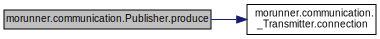
\includegraphics[width=350pt]{classmorunner_1_1communication_1_1Publisher_a31e6bd7d0f60bfde37c026ddd55ff8b6_cgraph}
\end{center}
\end{figure}




The documentation for this class was generated from the following file\+:\begin{DoxyCompactItemize}
\item 
src/morunner/\hyperlink{communication_8py}{communication.\+py}\end{DoxyCompactItemize}

\hypertarget{classmorunner_1_1registry_1_1Registry}{}\section{morunner.\+registry.\+Registry Class Reference}
\label{classmorunner_1_1registry_1_1Registry}\index{morunner.\+registry.\+Registry@{morunner.\+registry.\+Registry}}


Inheritance diagram for morunner.\+registry.\+Registry\+:
\nopagebreak
\begin{figure}[H]
\begin{center}
\leavevmode
\includegraphics[width=212pt]{classmorunner_1_1registry_1_1Registry__inherit__graph}
\end{center}
\end{figure}


Collaboration diagram for morunner.\+registry.\+Registry\+:
\nopagebreak
\begin{figure}[H]
\begin{center}
\leavevmode
\includegraphics[width=212pt]{classmorunner_1_1registry_1_1Registry__coll__graph}
\end{center}
\end{figure}
\subsection*{Public Member Functions}
\begin{DoxyCompactItemize}
\item 
def \hyperlink{classmorunner_1_1registry_1_1Registry_a642af4ac15c0399e28377ca8bebeefef}{\+\_\+\+\_\+init\+\_\+\+\_\+} (self)
\end{DoxyCompactItemize}
\subsection*{Public Attributes}
\begin{DoxyCompactItemize}
\item 
\hyperlink{classmorunner_1_1registry_1_1Registry_a81f0b9c25ffd437f3b93d87e28211a6f}{breaks}
\item 
\hyperlink{classmorunner_1_1registry_1_1Registry_a526c4dd0693ed9206da10968a73f1ec6}{broadcaster}
\end{DoxyCompactItemize}


\subsection{Detailed Description}


Definition at line 7 of file registry.\+py.



\subsection{Constructor \& Destructor Documentation}
\hypertarget{classmorunner_1_1registry_1_1Registry_a642af4ac15c0399e28377ca8bebeefef}{}\index{morunner\+::registry\+::\+Registry@{morunner\+::registry\+::\+Registry}!\+\_\+\+\_\+init\+\_\+\+\_\+@{\+\_\+\+\_\+init\+\_\+\+\_\+}}
\index{\+\_\+\+\_\+init\+\_\+\+\_\+@{\+\_\+\+\_\+init\+\_\+\+\_\+}!morunner\+::registry\+::\+Registry@{morunner\+::registry\+::\+Registry}}
\subsubsection[{\+\_\+\+\_\+init\+\_\+\+\_\+(self)}]{\setlength{\rightskip}{0pt plus 5cm}def morunner.\+registry.\+Registry.\+\_\+\+\_\+init\+\_\+\+\_\+ (
\begin{DoxyParamCaption}
\item[{}]{self}
\end{DoxyParamCaption}
)}\label{classmorunner_1_1registry_1_1Registry_a642af4ac15c0399e28377ca8bebeefef}


Definition at line 9 of file registry.\+py.


\begin{DoxyCode}
9     \textcolor{keyword}{def }\hyperlink{classmorunner_1_1registry_1_1Registry_a642af4ac15c0399e28377ca8bebeefef}{\_\_init\_\_}(self):
10         self.\hyperlink{classmorunner_1_1registry_1_1Registry_a81f0b9c25ffd437f3b93d87e28211a6f}{breaks} = dict()
11         self.\hyperlink{classmorunner_1_1registry_1_1Registry_a526c4dd0693ed9206da10968a73f1ec6}{broadcaster} = \hyperlink{classmorunner_1_1communication_1_1Broadcaster}{communication.Broadcaster}()
12         self.
13 \end{DoxyCode}


\subsection{Member Data Documentation}
\hypertarget{classmorunner_1_1registry_1_1Registry_a81f0b9c25ffd437f3b93d87e28211a6f}{}\index{morunner\+::registry\+::\+Registry@{morunner\+::registry\+::\+Registry}!breaks@{breaks}}
\index{breaks@{breaks}!morunner\+::registry\+::\+Registry@{morunner\+::registry\+::\+Registry}}
\subsubsection[{breaks}]{\setlength{\rightskip}{0pt plus 5cm}morunner.\+registry.\+Registry.\+breaks}\label{classmorunner_1_1registry_1_1Registry_a81f0b9c25ffd437f3b93d87e28211a6f}


Definition at line 10 of file registry.\+py.

\hypertarget{classmorunner_1_1registry_1_1Registry_a526c4dd0693ed9206da10968a73f1ec6}{}\index{morunner\+::registry\+::\+Registry@{morunner\+::registry\+::\+Registry}!broadcaster@{broadcaster}}
\index{broadcaster@{broadcaster}!morunner\+::registry\+::\+Registry@{morunner\+::registry\+::\+Registry}}
\subsubsection[{broadcaster}]{\setlength{\rightskip}{0pt plus 5cm}morunner.\+registry.\+Registry.\+broadcaster}\label{classmorunner_1_1registry_1_1Registry_a526c4dd0693ed9206da10968a73f1ec6}


Definition at line 11 of file registry.\+py.



The documentation for this class was generated from the following file\+:\begin{DoxyCompactItemize}
\item 
src/morunner/\hyperlink{registry_8py}{registry.\+py}\end{DoxyCompactItemize}

\hypertarget{classmorunner_1_1communication_1_1Subject}{}\section{morunner.\+communication.\+Subject Class Reference}
\label{classmorunner_1_1communication_1_1Subject}\index{morunner.\+communication.\+Subject@{morunner.\+communication.\+Subject}}


Inheritance diagram for morunner.\+communication.\+Subject\+:
\nopagebreak
\begin{figure}[H]
\begin{center}
\leavevmode
\includegraphics[width=242pt]{classmorunner_1_1communication_1_1Subject__inherit__graph}
\end{center}
\end{figure}


Collaboration diagram for morunner.\+communication.\+Subject\+:
\nopagebreak
\begin{figure}[H]
\begin{center}
\leavevmode
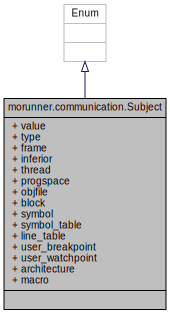
\includegraphics[width=242pt]{classmorunner_1_1communication_1_1Subject__coll__graph}
\end{center}
\end{figure}
\subsection*{Static Public Attributes}
\begin{DoxyCompactItemize}
\item 
int \hyperlink{classmorunner_1_1communication_1_1Subject_ab43ed6150da716dccc34f12e9ea60eb9}{value} = 0
\item 
int \hyperlink{classmorunner_1_1communication_1_1Subject_a14af2bb1b6e526ffdca900d719cbf169}{type} = 1
\item 
int \hyperlink{classmorunner_1_1communication_1_1Subject_a096a79c71387142b11d5d536bda224ef}{frame} = 2
\item 
int \hyperlink{classmorunner_1_1communication_1_1Subject_a50b156272f64da73b4b8799847578da8}{inferior} = 3
\item 
int \hyperlink{classmorunner_1_1communication_1_1Subject_af7cf15dff5836ca6019013f443065bf0}{thread} = 4
\item 
int \hyperlink{classmorunner_1_1communication_1_1Subject_ab8f9822ebaf741ec0a2c549dd05c32b6}{progspace} = 5
\item 
int \hyperlink{classmorunner_1_1communication_1_1Subject_ad1990b04607b95087b9fbd3838f61db6}{objfile} = 6
\item 
int \hyperlink{classmorunner_1_1communication_1_1Subject_a4164b6a9955ed4dcd4710a50b28bbeac}{block} = 7
\item 
int \hyperlink{classmorunner_1_1communication_1_1Subject_a47691d34d36ac6b6009eebeb30a137f7}{symbol} = 8
\item 
int \hyperlink{classmorunner_1_1communication_1_1Subject_a2d1c9aa83c85cbdf689428420f72c002}{symbol\+\_\+table} = 9
\item 
int \hyperlink{classmorunner_1_1communication_1_1Subject_aea4d95ee9a997eeb2368bf8665837517}{line\+\_\+table} = 10
\item 
int \hyperlink{classmorunner_1_1communication_1_1Subject_a1e3fcdc8be94d51e906d17e7c0235556}{user\+\_\+breakpoint} = 11
\item 
int \hyperlink{classmorunner_1_1communication_1_1Subject_abbc303b6440251f7eb90012d1d1e12b9}{user\+\_\+watchpoint} = 12
\item 
int \hyperlink{classmorunner_1_1communication_1_1Subject_ae8f2eb6f002dc62290238d42280975a0}{architecture} = 13
\item 
int \hyperlink{classmorunner_1_1communication_1_1Subject_a632bc45f41b3da11876076c3ec353e21}{macro} = 14
\end{DoxyCompactItemize}


\subsection{Detailed Description}
\begin{DoxyVerb}The list of valid subject codes for messages.
\end{DoxyVerb}
 

Definition at line 69 of file communication.\+py.



\subsection{Member Data Documentation}
\hypertarget{classmorunner_1_1communication_1_1Subject_ae8f2eb6f002dc62290238d42280975a0}{}\index{morunner\+::communication\+::\+Subject@{morunner\+::communication\+::\+Subject}!architecture@{architecture}}
\index{architecture@{architecture}!morunner\+::communication\+::\+Subject@{morunner\+::communication\+::\+Subject}}
\subsubsection[{architecture}]{\setlength{\rightskip}{0pt plus 5cm}int morunner.\+communication.\+Subject.\+architecture = 13\hspace{0.3cm}{\ttfamily [static]}}\label{classmorunner_1_1communication_1_1Subject_ae8f2eb6f002dc62290238d42280975a0}


Definition at line 87 of file communication.\+py.

\hypertarget{classmorunner_1_1communication_1_1Subject_a4164b6a9955ed4dcd4710a50b28bbeac}{}\index{morunner\+::communication\+::\+Subject@{morunner\+::communication\+::\+Subject}!block@{block}}
\index{block@{block}!morunner\+::communication\+::\+Subject@{morunner\+::communication\+::\+Subject}}
\subsubsection[{block}]{\setlength{\rightskip}{0pt plus 5cm}int morunner.\+communication.\+Subject.\+block = 7\hspace{0.3cm}{\ttfamily [static]}}\label{classmorunner_1_1communication_1_1Subject_a4164b6a9955ed4dcd4710a50b28bbeac}


Definition at line 81 of file communication.\+py.

\hypertarget{classmorunner_1_1communication_1_1Subject_a096a79c71387142b11d5d536bda224ef}{}\index{morunner\+::communication\+::\+Subject@{morunner\+::communication\+::\+Subject}!frame@{frame}}
\index{frame@{frame}!morunner\+::communication\+::\+Subject@{morunner\+::communication\+::\+Subject}}
\subsubsection[{frame}]{\setlength{\rightskip}{0pt plus 5cm}int morunner.\+communication.\+Subject.\+frame = 2\hspace{0.3cm}{\ttfamily [static]}}\label{classmorunner_1_1communication_1_1Subject_a096a79c71387142b11d5d536bda224ef}


Definition at line 76 of file communication.\+py.

\hypertarget{classmorunner_1_1communication_1_1Subject_a50b156272f64da73b4b8799847578da8}{}\index{morunner\+::communication\+::\+Subject@{morunner\+::communication\+::\+Subject}!inferior@{inferior}}
\index{inferior@{inferior}!morunner\+::communication\+::\+Subject@{morunner\+::communication\+::\+Subject}}
\subsubsection[{inferior}]{\setlength{\rightskip}{0pt plus 5cm}int morunner.\+communication.\+Subject.\+inferior = 3\hspace{0.3cm}{\ttfamily [static]}}\label{classmorunner_1_1communication_1_1Subject_a50b156272f64da73b4b8799847578da8}


Definition at line 77 of file communication.\+py.

\hypertarget{classmorunner_1_1communication_1_1Subject_aea4d95ee9a997eeb2368bf8665837517}{}\index{morunner\+::communication\+::\+Subject@{morunner\+::communication\+::\+Subject}!line\+\_\+table@{line\+\_\+table}}
\index{line\+\_\+table@{line\+\_\+table}!morunner\+::communication\+::\+Subject@{morunner\+::communication\+::\+Subject}}
\subsubsection[{line\+\_\+table}]{\setlength{\rightskip}{0pt plus 5cm}int morunner.\+communication.\+Subject.\+line\+\_\+table = 10\hspace{0.3cm}{\ttfamily [static]}}\label{classmorunner_1_1communication_1_1Subject_aea4d95ee9a997eeb2368bf8665837517}


Definition at line 84 of file communication.\+py.

\hypertarget{classmorunner_1_1communication_1_1Subject_a632bc45f41b3da11876076c3ec353e21}{}\index{morunner\+::communication\+::\+Subject@{morunner\+::communication\+::\+Subject}!macro@{macro}}
\index{macro@{macro}!morunner\+::communication\+::\+Subject@{morunner\+::communication\+::\+Subject}}
\subsubsection[{macro}]{\setlength{\rightskip}{0pt plus 5cm}int morunner.\+communication.\+Subject.\+macro = 14\hspace{0.3cm}{\ttfamily [static]}}\label{classmorunner_1_1communication_1_1Subject_a632bc45f41b3da11876076c3ec353e21}


Definition at line 88 of file communication.\+py.

\hypertarget{classmorunner_1_1communication_1_1Subject_ad1990b04607b95087b9fbd3838f61db6}{}\index{morunner\+::communication\+::\+Subject@{morunner\+::communication\+::\+Subject}!objfile@{objfile}}
\index{objfile@{objfile}!morunner\+::communication\+::\+Subject@{morunner\+::communication\+::\+Subject}}
\subsubsection[{objfile}]{\setlength{\rightskip}{0pt plus 5cm}int morunner.\+communication.\+Subject.\+objfile = 6\hspace{0.3cm}{\ttfamily [static]}}\label{classmorunner_1_1communication_1_1Subject_ad1990b04607b95087b9fbd3838f61db6}


Definition at line 80 of file communication.\+py.

\hypertarget{classmorunner_1_1communication_1_1Subject_ab8f9822ebaf741ec0a2c549dd05c32b6}{}\index{morunner\+::communication\+::\+Subject@{morunner\+::communication\+::\+Subject}!progspace@{progspace}}
\index{progspace@{progspace}!morunner\+::communication\+::\+Subject@{morunner\+::communication\+::\+Subject}}
\subsubsection[{progspace}]{\setlength{\rightskip}{0pt plus 5cm}int morunner.\+communication.\+Subject.\+progspace = 5\hspace{0.3cm}{\ttfamily [static]}}\label{classmorunner_1_1communication_1_1Subject_ab8f9822ebaf741ec0a2c549dd05c32b6}


Definition at line 79 of file communication.\+py.

\hypertarget{classmorunner_1_1communication_1_1Subject_a47691d34d36ac6b6009eebeb30a137f7}{}\index{morunner\+::communication\+::\+Subject@{morunner\+::communication\+::\+Subject}!symbol@{symbol}}
\index{symbol@{symbol}!morunner\+::communication\+::\+Subject@{morunner\+::communication\+::\+Subject}}
\subsubsection[{symbol}]{\setlength{\rightskip}{0pt plus 5cm}int morunner.\+communication.\+Subject.\+symbol = 8\hspace{0.3cm}{\ttfamily [static]}}\label{classmorunner_1_1communication_1_1Subject_a47691d34d36ac6b6009eebeb30a137f7}


Definition at line 82 of file communication.\+py.

\hypertarget{classmorunner_1_1communication_1_1Subject_a2d1c9aa83c85cbdf689428420f72c002}{}\index{morunner\+::communication\+::\+Subject@{morunner\+::communication\+::\+Subject}!symbol\+\_\+table@{symbol\+\_\+table}}
\index{symbol\+\_\+table@{symbol\+\_\+table}!morunner\+::communication\+::\+Subject@{morunner\+::communication\+::\+Subject}}
\subsubsection[{symbol\+\_\+table}]{\setlength{\rightskip}{0pt plus 5cm}int morunner.\+communication.\+Subject.\+symbol\+\_\+table = 9\hspace{0.3cm}{\ttfamily [static]}}\label{classmorunner_1_1communication_1_1Subject_a2d1c9aa83c85cbdf689428420f72c002}


Definition at line 83 of file communication.\+py.

\hypertarget{classmorunner_1_1communication_1_1Subject_af7cf15dff5836ca6019013f443065bf0}{}\index{morunner\+::communication\+::\+Subject@{morunner\+::communication\+::\+Subject}!thread@{thread}}
\index{thread@{thread}!morunner\+::communication\+::\+Subject@{morunner\+::communication\+::\+Subject}}
\subsubsection[{thread}]{\setlength{\rightskip}{0pt plus 5cm}int morunner.\+communication.\+Subject.\+thread = 4\hspace{0.3cm}{\ttfamily [static]}}\label{classmorunner_1_1communication_1_1Subject_af7cf15dff5836ca6019013f443065bf0}


Definition at line 78 of file communication.\+py.

\hypertarget{classmorunner_1_1communication_1_1Subject_a14af2bb1b6e526ffdca900d719cbf169}{}\index{morunner\+::communication\+::\+Subject@{morunner\+::communication\+::\+Subject}!type@{type}}
\index{type@{type}!morunner\+::communication\+::\+Subject@{morunner\+::communication\+::\+Subject}}
\subsubsection[{type}]{\setlength{\rightskip}{0pt plus 5cm}int morunner.\+communication.\+Subject.\+type = 1\hspace{0.3cm}{\ttfamily [static]}}\label{classmorunner_1_1communication_1_1Subject_a14af2bb1b6e526ffdca900d719cbf169}


Definition at line 75 of file communication.\+py.

\hypertarget{classmorunner_1_1communication_1_1Subject_a1e3fcdc8be94d51e906d17e7c0235556}{}\index{morunner\+::communication\+::\+Subject@{morunner\+::communication\+::\+Subject}!user\+\_\+breakpoint@{user\+\_\+breakpoint}}
\index{user\+\_\+breakpoint@{user\+\_\+breakpoint}!morunner\+::communication\+::\+Subject@{morunner\+::communication\+::\+Subject}}
\subsubsection[{user\+\_\+breakpoint}]{\setlength{\rightskip}{0pt plus 5cm}int morunner.\+communication.\+Subject.\+user\+\_\+breakpoint = 11\hspace{0.3cm}{\ttfamily [static]}}\label{classmorunner_1_1communication_1_1Subject_a1e3fcdc8be94d51e906d17e7c0235556}


Definition at line 85 of file communication.\+py.

\hypertarget{classmorunner_1_1communication_1_1Subject_abbc303b6440251f7eb90012d1d1e12b9}{}\index{morunner\+::communication\+::\+Subject@{morunner\+::communication\+::\+Subject}!user\+\_\+watchpoint@{user\+\_\+watchpoint}}
\index{user\+\_\+watchpoint@{user\+\_\+watchpoint}!morunner\+::communication\+::\+Subject@{morunner\+::communication\+::\+Subject}}
\subsubsection[{user\+\_\+watchpoint}]{\setlength{\rightskip}{0pt plus 5cm}int morunner.\+communication.\+Subject.\+user\+\_\+watchpoint = 12\hspace{0.3cm}{\ttfamily [static]}}\label{classmorunner_1_1communication_1_1Subject_abbc303b6440251f7eb90012d1d1e12b9}


Definition at line 86 of file communication.\+py.

\hypertarget{classmorunner_1_1communication_1_1Subject_ab43ed6150da716dccc34f12e9ea60eb9}{}\index{morunner\+::communication\+::\+Subject@{morunner\+::communication\+::\+Subject}!value@{value}}
\index{value@{value}!morunner\+::communication\+::\+Subject@{morunner\+::communication\+::\+Subject}}
\subsubsection[{value}]{\setlength{\rightskip}{0pt plus 5cm}int morunner.\+communication.\+Subject.\+value = 0\hspace{0.3cm}{\ttfamily [static]}}\label{classmorunner_1_1communication_1_1Subject_ab43ed6150da716dccc34f12e9ea60eb9}


Definition at line 74 of file communication.\+py.



The documentation for this class was generated from the following file\+:\begin{DoxyCompactItemize}
\item 
src/morunner/\hyperlink{communication_8py}{communication.\+py}\end{DoxyCompactItemize}

\hypertarget{classmorunner_1_1communication_1_1Subscriber}{}\section{morunner.\+communication.\+Subscriber Class Reference}
\label{classmorunner_1_1communication_1_1Subscriber}\index{morunner.\+communication.\+Subscriber@{morunner.\+communication.\+Subscriber}}


Inheritance diagram for morunner.\+communication.\+Subscriber\+:
\nopagebreak
\begin{figure}[H]
\begin{center}
\leavevmode
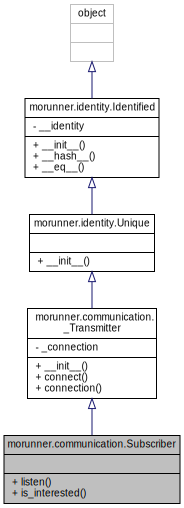
\includegraphics[height=550pt]{classmorunner_1_1communication_1_1Subscriber__inherit__graph}
\end{center}
\end{figure}


Collaboration diagram for morunner.\+communication.\+Subscriber\+:
\nopagebreak
\begin{figure}[H]
\begin{center}
\leavevmode
\includegraphics[height=550pt]{classmorunner_1_1communication_1_1Subscriber__coll__graph}
\end{center}
\end{figure}
\subsection*{Public Member Functions}
\begin{DoxyCompactItemize}
\item 
def \hyperlink{classmorunner_1_1communication_1_1Subscriber_ad16726eaf7536b090444a89c1d8b047b}{listen} (self)
\item 
def \hyperlink{classmorunner_1_1communication_1_1Subscriber_a1d8ab4ea99db86ba77176f6f282db254}{is\+\_\+interested}
\end{DoxyCompactItemize}


\subsection{Detailed Description}


Definition at line 153 of file communication.\+py.



\subsection{Member Function Documentation}
\hypertarget{classmorunner_1_1communication_1_1Subscriber_a1d8ab4ea99db86ba77176f6f282db254}{}\index{morunner\+::communication\+::\+Subscriber@{morunner\+::communication\+::\+Subscriber}!is\+\_\+interested@{is\+\_\+interested}}
\index{is\+\_\+interested@{is\+\_\+interested}!morunner\+::communication\+::\+Subscriber@{morunner\+::communication\+::\+Subscriber}}
\subsubsection[{is\+\_\+interested}]{\setlength{\rightskip}{0pt plus 5cm}def morunner.\+communication.\+Subscriber.\+is\+\_\+interested (
\begin{DoxyParamCaption}
\item[{}]{cls, }
\item[{}]{message}
\end{DoxyParamCaption}
)}\label{classmorunner_1_1communication_1_1Subscriber_a1d8ab4ea99db86ba77176f6f282db254}


Definition at line 166 of file communication.\+py.


\begin{DoxyCode}
166     \textcolor{keyword}{def }\hyperlink{classmorunner_1_1communication_1_1Subscriber_a1d8ab4ea99db86ba77176f6f282db254}{is\_interested}(cls, message: Message) -> bool:
167         \textcolor{stringliteral}{"""}
168 \textcolor{stringliteral}{        Override this method to make your subscriber only collect the messages}
169 \textcolor{stringliteral}{        it cares about.}
170 \textcolor{stringliteral}{        """}
171         \textcolor{keywordflow}{raise} NotImplementedError(\textcolor{stringliteral}{"Subscriber must be subclassed!"})
172 
173 
\end{DoxyCode}
\hypertarget{classmorunner_1_1communication_1_1Subscriber_ad16726eaf7536b090444a89c1d8b047b}{}\index{morunner\+::communication\+::\+Subscriber@{morunner\+::communication\+::\+Subscriber}!listen@{listen}}
\index{listen@{listen}!morunner\+::communication\+::\+Subscriber@{morunner\+::communication\+::\+Subscriber}}
\subsubsection[{listen(self)}]{\setlength{\rightskip}{0pt plus 5cm}def morunner.\+communication.\+Subscriber.\+listen (
\begin{DoxyParamCaption}
\item[{}]{self, }
\item[{}]{None}
\end{DoxyParamCaption}
)}\label{classmorunner_1_1communication_1_1Subscriber_ad16726eaf7536b090444a89c1d8b047b}
\begin{DoxyVerb}Listen for messages from the broadcaster.
\end{DoxyVerb}
 

Definition at line 155 of file communication.\+py.



References morunner.\+communication.\+\_\+\+Transmitter.\+connection().


\begin{DoxyCode}
155     \textcolor{keyword}{def }\hyperlink{classmorunner_1_1communication_1_1Subscriber_ad16726eaf7536b090444a89c1d8b047b}{listen}(self) -> None:
156         \textcolor{stringliteral}{"""}
157 \textcolor{stringliteral}{        Listen for messages from the broadcaster.}
158 \textcolor{stringliteral}{        """}
159         \textcolor{keywordflow}{while} self.\hyperlink{classmorunner_1_1communication_1_1__Transmitter_a054317d3dbeecd42d6bbb81612d67ea5}{connection}:
160             \textcolor{keywordflow}{for} ready\_connection \textcolor{keywordflow}{in} multiprocessing.connection.wait([self.
      \hyperlink{classmorunner_1_1communication_1_1__Transmitter_a054317d3dbeecd42d6bbb81612d67ea5}{connection}]):
161                 message = ready\_connection.recv()
162                 \textcolor{comment}{# TODO: Deal with message}
163                 \textcolor{comment}{# print("got a ", x)}
164 
\end{DoxyCode}


Here is the call graph for this function\+:
\nopagebreak
\begin{figure}[H]
\begin{center}
\leavevmode
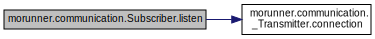
\includegraphics[width=350pt]{classmorunner_1_1communication_1_1Subscriber_ad16726eaf7536b090444a89c1d8b047b_cgraph}
\end{center}
\end{figure}




The documentation for this class was generated from the following file\+:\begin{DoxyCompactItemize}
\item 
src/morunner/\hyperlink{communication_8py}{communication.\+py}\end{DoxyCompactItemize}

\hypertarget{classmorunner_1_1break_1_1Task}{}\section{morunner.\+break.\+Task Class Reference}
\label{classmorunner_1_1break_1_1Task}\index{morunner.\+break.\+Task@{morunner.\+break.\+Task}}


Inheritance diagram for morunner.\+break.\+Task\+:
\nopagebreak
\begin{figure}[H]
\begin{center}
\leavevmode
\includegraphics[width=189pt]{classmorunner_1_1break_1_1Task__inherit__graph}
\end{center}
\end{figure}


Collaboration diagram for morunner.\+break.\+Task\+:
\nopagebreak
\begin{figure}[H]
\begin{center}
\leavevmode
\includegraphics[width=189pt]{classmorunner_1_1break_1_1Task__coll__graph}
\end{center}
\end{figure}
\subsection*{Public Member Functions}
\begin{DoxyCompactItemize}
\item 
def \hyperlink{classmorunner_1_1break_1_1Task_af3aaf4517e4358ea2164780cd32afff6}{\+\_\+\+\_\+init\+\_\+\+\_\+} (self, registry)
\end{DoxyCompactItemize}


\subsection{Detailed Description}


Definition at line 24 of file break.\+py.



\subsection{Constructor \& Destructor Documentation}
\hypertarget{classmorunner_1_1break_1_1Task_af3aaf4517e4358ea2164780cd32afff6}{}\index{morunner\+::break\+::\+Task@{morunner\+::break\+::\+Task}!\+\_\+\+\_\+init\+\_\+\+\_\+@{\+\_\+\+\_\+init\+\_\+\+\_\+}}
\index{\+\_\+\+\_\+init\+\_\+\+\_\+@{\+\_\+\+\_\+init\+\_\+\+\_\+}!morunner\+::break\+::\+Task@{morunner\+::break\+::\+Task}}
\subsubsection[{\+\_\+\+\_\+init\+\_\+\+\_\+(self, registry)}]{\setlength{\rightskip}{0pt plus 5cm}def morunner.\+break.\+Task.\+\_\+\+\_\+init\+\_\+\+\_\+ (
\begin{DoxyParamCaption}
\item[{}]{self, }
\item[{}]{registry}
\end{DoxyParamCaption}
)}\label{classmorunner_1_1break_1_1Task_af3aaf4517e4358ea2164780cd32afff6}


Definition at line 26 of file break.\+py.


\begin{DoxyCode}
26     \textcolor{keyword}{def }\hyperlink{classmorunner_1_1break_1_1Task_af3aaf4517e4358ea2164780cd32afff6}{\_\_init\_\_}(self, registry):
27 
28 
29 
30 
\end{DoxyCode}


The documentation for this class was generated from the following file\+:\begin{DoxyCompactItemize}
\item 
src/morunner/\hyperlink{break_8py}{break.\+py}\end{DoxyCompactItemize}

\hypertarget{classmorunner_1_1identity_1_1Unique}{}\section{morunner.\+identity.\+Unique Class Reference}
\label{classmorunner_1_1identity_1_1Unique}\index{morunner.\+identity.\+Unique@{morunner.\+identity.\+Unique}}


Inheritance diagram for morunner.\+identity.\+Unique\+:
\nopagebreak
\begin{figure}[H]
\begin{center}
\leavevmode
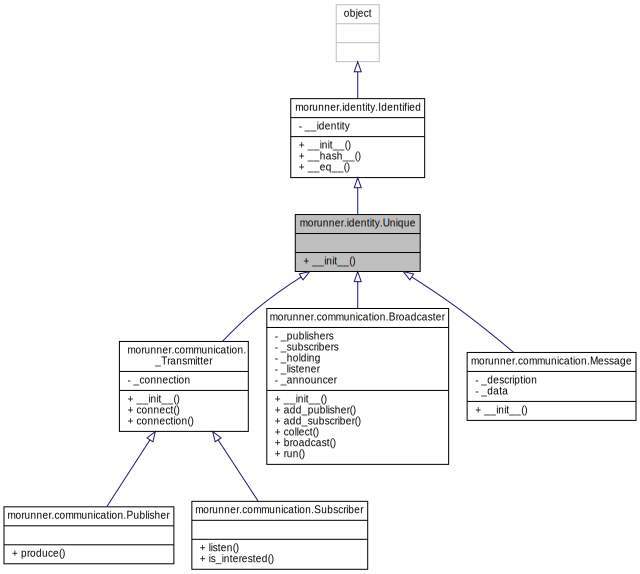
\includegraphics[width=350pt]{classmorunner_1_1identity_1_1Unique__inherit__graph}
\end{center}
\end{figure}


Collaboration diagram for morunner.\+identity.\+Unique\+:
\nopagebreak
\begin{figure}[H]
\begin{center}
\leavevmode
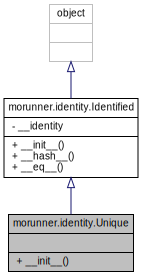
\includegraphics[width=214pt]{classmorunner_1_1identity_1_1Unique__coll__graph}
\end{center}
\end{figure}
\subsection*{Public Member Functions}
\begin{DoxyCompactItemize}
\item 
def \hyperlink{classmorunner_1_1identity_1_1Unique_af40fb103e03b1f5ae87e3050ff1a903b}{\+\_\+\+\_\+init\+\_\+\+\_\+} (self)
\end{DoxyCompactItemize}


\subsection{Detailed Description}
\begin{DoxyVerb}Assigns a (globally) unique id tag to every instance in __init__.
\end{DoxyVerb}
 

Definition at line 58 of file identity.\+py.



\subsection{Constructor \& Destructor Documentation}
\hypertarget{classmorunner_1_1identity_1_1Unique_af40fb103e03b1f5ae87e3050ff1a903b}{}\index{morunner\+::identity\+::\+Unique@{morunner\+::identity\+::\+Unique}!\+\_\+\+\_\+init\+\_\+\+\_\+@{\+\_\+\+\_\+init\+\_\+\+\_\+}}
\index{\+\_\+\+\_\+init\+\_\+\+\_\+@{\+\_\+\+\_\+init\+\_\+\+\_\+}!morunner\+::identity\+::\+Unique@{morunner\+::identity\+::\+Unique}}
\subsubsection[{\+\_\+\+\_\+init\+\_\+\+\_\+(self)}]{\setlength{\rightskip}{0pt plus 5cm}def morunner.\+identity.\+Unique.\+\_\+\+\_\+init\+\_\+\+\_\+ (
\begin{DoxyParamCaption}
\item[{}]{self, }
\item[{}]{None}
\end{DoxyParamCaption}
)}\label{classmorunner_1_1identity_1_1Unique_af40fb103e03b1f5ae87e3050ff1a903b}
\begin{DoxyVerb}Passes a function (currently uuid.uuid4) to the Identified.__init__
call.  This has the effect of giving every instance of unique a
different hash value.
\end{DoxyVerb}
 

Definition at line 63 of file identity.\+py.


\begin{DoxyCode}
63     \textcolor{keyword}{def }\hyperlink{classmorunner_1_1identity_1_1Unique_af40fb103e03b1f5ae87e3050ff1a903b}{\_\_init\_\_}(self) -> None:
64         \textcolor{stringliteral}{"""}
65 \textcolor{stringliteral}{        Passes a function (currently uuid.uuid4) to the Identified.\_\_init\_\_}
66 \textcolor{stringliteral}{        call.  This has the effect of giving every instance of unique a}
67 \textcolor{stringliteral}{        different hash value.}
68 \textcolor{stringliteral}{        """}
69         super(Unique, self).\hyperlink{classmorunner_1_1identity_1_1Unique_af40fb103e03b1f5ae87e3050ff1a903b}{\_\_init\_\_}(uuid.uuid4)
70 \end{DoxyCode}


The documentation for this class was generated from the following file\+:\begin{DoxyCompactItemize}
\item 
src/morunner/\hyperlink{identity_8py}{identity.\+py}\end{DoxyCompactItemize}

\chapter{File Documentation}
\hypertarget{____init_____8py}{}\section{src/morunner/\+\_\+\+\_\+init\+\_\+\+\_\+.py File Reference}
\label{____init_____8py}\index{src/morunner/\+\_\+\+\_\+init\+\_\+\+\_\+.\+py@{src/morunner/\+\_\+\+\_\+init\+\_\+\+\_\+.\+py}}
\subsection*{Namespaces}
\begin{DoxyCompactItemize}
\item 
 \hyperlink{namespacemorunner}{morunner}
\end{DoxyCompactItemize}

\hypertarget{break_8py}{}\section{src/morunner/break.py File Reference}
\label{break_8py}\index{src/morunner/break.\+py@{src/morunner/break.\+py}}
\subsection*{Classes}
\begin{DoxyCompactItemize}
\item 
class \hyperlink{classmorunner_1_1break_1_1Task}{morunner.\+break.\+Task}
\item 
class \hyperlink{classmorunner_1_1break_1_1Break}{morunner.\+break.\+Break}
\end{DoxyCompactItemize}
\subsection*{Namespaces}
\begin{DoxyCompactItemize}
\item 
 \hyperlink{namespacemorunner_1_1break}{morunner.\+break}
\end{DoxyCompactItemize}
\subsection*{Variables}
\begin{DoxyCompactItemize}
\item 
tuple \hyperlink{namespacemorunner_1_1break_a8ae952471ddccae191c37b56975d1f77}{morunner.\+break.\+Break\+Condition}
\end{DoxyCompactItemize}

\hypertarget{communication_8py}{}\section{src/morunner/communication.py File Reference}
\label{communication_8py}\index{src/morunner/communication.\+py@{src/morunner/communication.\+py}}
\subsection*{Classes}
\begin{DoxyCompactItemize}
\item 
class \hyperlink{classmorunner_1_1communication_1_1Action}{morunner.\+communication.\+Action}
\item 
class \hyperlink{classmorunner_1_1communication_1_1Subject}{morunner.\+communication.\+Subject}
\item 
class \hyperlink{classmorunner_1_1communication_1_1MessageDescription}{morunner.\+communication.\+Message\+Description}
\item 
class \hyperlink{classmorunner_1_1communication_1_1Message}{morunner.\+communication.\+Message}
\item 
class \hyperlink{classmorunner_1_1communication_1_1__Transmitter}{morunner.\+communication.\+\_\+\+Transmitter}
\item 
class \hyperlink{classmorunner_1_1communication_1_1Publisher}{morunner.\+communication.\+Publisher}
\item 
class \hyperlink{classmorunner_1_1communication_1_1Subscriber}{morunner.\+communication.\+Subscriber}
\item 
class \hyperlink{classmorunner_1_1communication_1_1Broadcaster}{morunner.\+communication.\+Broadcaster}
\end{DoxyCompactItemize}
\subsection*{Namespaces}
\begin{DoxyCompactItemize}
\item 
 \hyperlink{namespacemorunner_1_1communication}{morunner.\+communication}
\end{DoxyCompactItemize}

\hypertarget{identity_8py}{}\section{src/morunner/identity.py File Reference}
\label{identity_8py}\index{src/morunner/identity.\+py@{src/morunner/identity.\+py}}
\subsection*{Classes}
\begin{DoxyCompactItemize}
\item 
class \hyperlink{classmorunner_1_1identity_1_1Identified}{morunner.\+identity.\+Identified}
\item 
class \hyperlink{classmorunner_1_1identity_1_1Unique}{morunner.\+identity.\+Unique}
\end{DoxyCompactItemize}
\subsection*{Namespaces}
\begin{DoxyCompactItemize}
\item 
 \hyperlink{namespacemorunner_1_1identity}{morunner.\+identity}
\end{DoxyCompactItemize}

\hypertarget{registry_8py}{}\section{src/morunner/registry.py File Reference}
\label{registry_8py}\index{src/morunner/registry.\+py@{src/morunner/registry.\+py}}
\subsection*{Classes}
\begin{DoxyCompactItemize}
\item 
class \hyperlink{classmorunner_1_1registry_1_1Registry}{morunner.\+registry.\+Registry}
\end{DoxyCompactItemize}
\subsection*{Namespaces}
\begin{DoxyCompactItemize}
\item 
 \hyperlink{namespacemorunner_1_1registry}{morunner.\+registry}
\end{DoxyCompactItemize}

%--- End generated contents ---

% Index
\backmatter
\newpage
\phantomsection
\clearemptydoublepage
\addcontentsline{toc}{chapter}{Index}
\printindex

\end{document}
